\documentclass[11pt]{article}
% Preamble of observational_classification.tex: packages, colours, the TikZ vocabulary of the figures, boxes, macros.
\usepackage[a4paper,margin=2.35cm]{geometry}
\usepackage[T1]{fontenc}
\usepackage[utf8]{inputenc}
\usepackage{lmodern}
\usepackage{microtype}
\usepackage{amsmath,amssymb,amsthm,mathtools}
\usepackage{booktabs,array,multirow}
\usepackage{enumitem}
\usepackage{float}
\usepackage[font=small,labelfont=bf]{caption}
\usepackage{xcolor}
\usepackage{tikz}
\usetikzlibrary{arrows.meta,positioning,calc,backgrounds,fit,shapes.geometric,decorations.pathreplacing}
\usepackage[most]{tcolorbox}
\usepackage[colorlinks=true,linkcolor=oiblue!80!black,citecolor=oigreen!70!black,urlcolor=oiblue!80!black]{hyperref}
\usepackage[capitalise,noabbrev]{cleveref}

% ---------------------------------------------------------------------------------------------------------------
% Colours: the Okabe-Ito palette, which stays distinguishable under the common colour-vision deficiencies.
% ---------------------------------------------------------------------------------------------------------------
\definecolor{oiorange}{RGB}{230,159,0}
\definecolor{oisky}{RGB}{86,180,233}
\definecolor{oigreen}{RGB}{0,158,115}
\definecolor{oiyellow}{RGB}{240,228,66}
\definecolor{oiblue}{RGB}{0,114,178}
\definecolor{oired}{RGB}{213,94,0}
\definecolor{oipurple}{RGB}{204,121,167}
\colorlet{qcol}{oipurple!82!black}      % quantum sources and what they send
\colorlet{ccol}{oiblue}                 % classical data handed out by a source
\colorlet{Cfill}{oisky!55}              % the part C that is split off
\colorlet{Dfill}{oigreen!38}            % the part D that sees C
\colorlet{splitcol}{oiorange}           % the source that is being split
\colorlet{dropcol}{oired}               % the edge that is dropped
\colorlet{premcol}{oiyellow!70}         % premeasurable nodes
\colorlet{neutral}{black!55}            % boxes and discs that carry no status

% ---------------------------------------------------------------------------------------------------------------
% TikZ vocabulary. A structure is drawn with \vn (visible node), \qs (quantum source), \feed (source to members)
% and \de (visible edge).
% ---------------------------------------------------------------------------------------------------------------
\tikzset{
  mdag/.style={>={Stealth[length=2.0mm,width=1.6mm]}, line cap=round, line join=round, font=\small},
  vis/.style={circle, draw=black, line width=0.7pt, fill=white, minimum size=6.6mm, inner sep=0pt, font=\small},
  Cn/.style={vis, fill=Cfill},
  Dn/.style={vis, fill=Dfill},
  pre/.style={vis, fill=premcol},
  src/.style={diamond, aspect=1, draw=qcol!75!black, line width=0.5pt, fill=qcol, minimum size=4.6mm, inner sep=0pt},
  splitsrc/.style={src, draw=splitcol!70!black, fill=splitcol},
  csrc/.style={src, draw=ccol!75!black, fill=ccol!65},
  edge/.style={->, line width=0.8pt, black},
  qedge/.style={->, line width=0.8pt, qcol},
  splitedge/.style={->, line width=0.8pt, splitcol!85!black},
  cedge/.style={->, line width=0.8pt, ccol, densely dashed},
  dropedge/.style={->, line width=0.9pt, dropcol, densely dashed},
  newedge/.style={->, line width=1.0pt, oigreen!75!black},
  faint/.style={opacity=0.28},
  lab/.style={font=\footnotesize, inner sep=1.5pt},
  rel/.style={font=\Large},
  tag/.style={font=\scriptsize\itshape, text=black!70},
}
\newcommand{\vn}[4][vis]{\node[#1] (#2) at (#3) {#4};}
\newcommand{\qs}[3][src]{\node[#1] (#2) at (#3) {};}
\newcommand{\feed}[3][qedge]{\foreach \target in {#3} {\draw[#1] (#2) -- (\target);}}
\newcommand{\de}[3][edge]{\draw[#1] (#2) -- (#3);}
% relation signs between two pictures
\newcommand{\equivsign}{\ensuremath{\boldsymbol{\equiv}}}
\newcommand{\nequivsign}{\ensuremath{\boldsymbol{\not\equiv}}}
\newcommand{\openequivsign}{\ensuremath{\overset{?}{\equiv}}}

% ---------------------------------------------------------------------------------------------------------------
% Boxes
% ---------------------------------------------------------------------------------------------------------------
\tcbset{boxbase/.style={enhanced, breakable, boxrule=0.8pt, arc=1.6mm, left=2.2mm, right=2.2mm, top=1.6mm,
                        bottom=1.6mm, fonttitle=\bfseries\small, before skip=9pt, after skip=9pt}}
\newtcolorbox{rulebox}[1]{boxbase, colback=oiblue!4, colframe=oiblue, title={#1}}
\newtcolorbox{validbox}[1]{boxbase, colback=oigreen!5, colframe=oigreen!85!black, title={\checkmark\enspace #1}}
\newtcolorbox{warnbox}[1]{boxbase, colback=oired!5, colframe=oired, title={$\boldsymbol{\times}$\enspace Not like this: #1}}
\newtcolorbox{openq}[1]{boxbase, colback=oiorange!7, colframe=oiorange!90!black, title={?\enspace Open: #1}}
\newtcolorbox{ideabox}[1]{boxbase, colback=black!3, colframe=black!55, title={#1}}

% ---------------------------------------------------------------------------------------------------------------
% Theorems
% ---------------------------------------------------------------------------------------------------------------
\theoremstyle{plain}
\newtheorem{theorem}{Theorem}
\newtheorem{lemma}[theorem]{Lemma}
\newtheorem{proposition}[theorem]{Proposition}
\newtheorem{corollary}[theorem]{Corollary}
\theoremstyle{definition}
\newtheorem{definition}[theorem]{Definition}
\newtheorem{example}[theorem]{Example}
\theoremstyle{remark}
\newtheorem{remark}[theorem]{Remark}

% ---------------------------------------------------------------------------------------------------------------
% Macros
% ---------------------------------------------------------------------------------------------------------------
\newcommand{\Q}{\mathcal{Q}}                         % quantum model set
\newcommand{\C}{\mathcal{C}}                         % classical model set
\newcommand{\G}{G}
\newcommand{\Pa}{\mathrm{Pa}}
\newcommand{\pa}{\mathrm{pa}}
\newcommand{\Tr}{\operatorname{Tr}}
\newcommand{\Hil}{\mathcal{H}}
\newcommand{\id}{\mathbf{1}}
\newcommand{\ket}[1]{\lvert #1\rangle}
\newcommand{\bra}[1]{\langle #1\rvert}
\newcommand{\proj}[1]{\lvert #1\rangle\!\langle #1\rvert}
\newcommand{\code}[1]{\texttt{#1}}
\newcommand{\str}[1]{\textsf{\small #1}}             % a structure in the repository's notation
\newcommand{\qeq}{\equiv_{\Q}}
\newcommand{\ceq}{\equiv_{\C}}
\newcommand{\AWS}{AWS}
\setlist{itemsep=2pt, topsep=4pt}
\setlength{\parskip}{4pt plus 1pt}
\setlength{\parindent}{0pt}


\title{\textbf{Observational equivalence rules for quantum causal models}\\[4pt]
\large what is proven, which classical rules fail, and what the classification buys}
\author{Notes for Marina, from the \code{mDAG-analysis} repository}
\date{November 2026}

\begin{document}
\maketitle

Which graphical changes preserve the distributions that independent quantum sources can produce?
The three moves in \cref{fig:glance} preserve both quantum and classical models. Their proofs use two
constructions: measuring a fixed observable at its source, and supplying a state for each possible visible
setting. Two Bell examples in \cref{sec:four-bell,sec:only-via} show how these moves extend a proof of a
quantum-classical gap to an entire class.

\section*{Summary}
\addcontentsline{toc}{section}{Summary}

\textbf{The question.} The census of quantum-classical gaps in this repository counts \emph{classes} of
structures that are proven to have the same quantum model set. Those classes are built from rules, and every rule
has to be valid for quantum sources. The rules were taken over from the classical theory, where a latent is a
random variable with a value. A quantum source has no value, only shares that are measured, and two of the three
classical rules use the value.

\textbf{The answer in one table.} A tick means proven; a cross means refuted by a counterexample in this note.

\begin{center}
\small
\renewcommand{\arraystretch}{1.25}
\begin{tabular}{@{}>{\raggedright\arraybackslash}p{3.0cm}>{\raggedright\arraybackslash}p{5.8cm}cc>{\raggedright\arraybackslash}p{2.5cm}@{}}
\toprule
\textbf{Rule} & \textbf{Hypothesis, in one line} & \textbf{Classical} & \textbf{Quantum} & \textbf{Where}\\
\midrule
Structural dominance & fewer edges or smaller sources allow fewer distributions
  & \checkmark & \checkmark & \cref{lem:monotone}\\
Face splitting, closed families & every source that touches the split-off part $C$ is split; the rest $D$ sees
  the outputs of $C$ and its visible parents & \checkmark & \checkmark & \cref{thm:split}\\
Face splitting, moderate and strong & as above, but a node of $C$ may also sit in an unsplit source that
  contains $D$ & \checkmark & $\boldsymbol{\times}$ & \cref{thm:sixnode}\\
Edge dropping, Rule A & the origin has no visible parent and a single source, which contains the target
  & \checkmark & \checkmark & \cref{thm:ruleA}\\
Edge dropping, Rule B & every other member of the origin's sources is premeasurable; the target sees the
  origin's inputs & \checkmark & \checkmark & \cref{thm:ruleB}\\
Edge dropping, the classical rule & the target sees the origin's visible parents and shares all its sources
  & \checkmark & $\boldsymbol{\times}$ & \cref{thm:hlp-settings,thm:hlp-four}\\
\bottomrule
\end{tabular}
\end{center}

\begin{figure}[H]
\centering
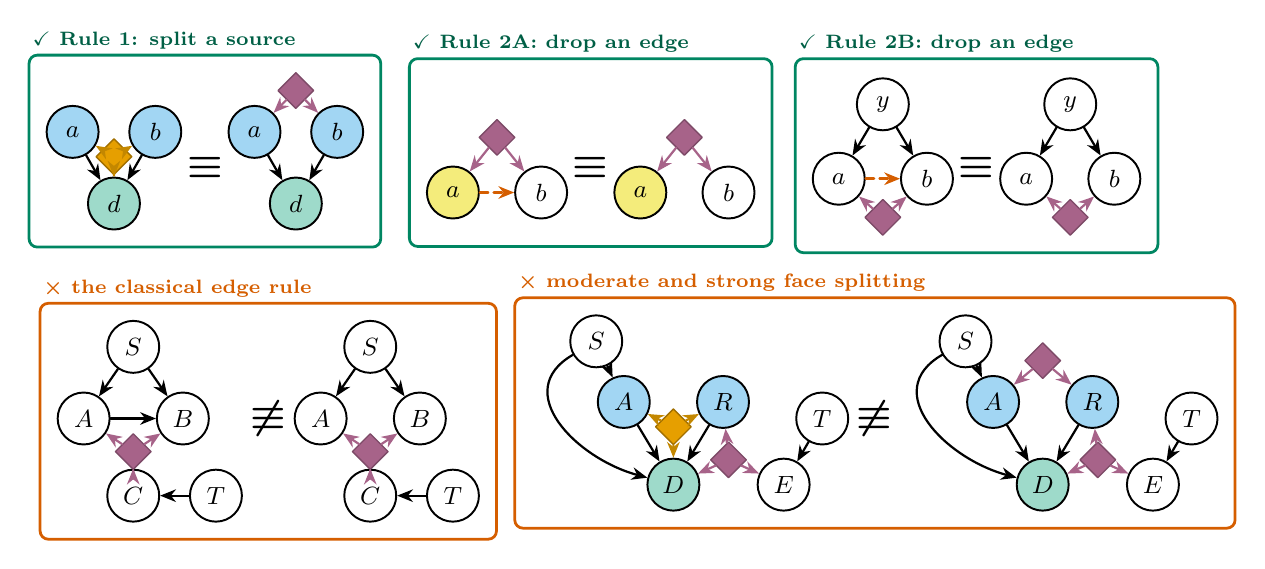
\begin{tikzpicture}[mdag,scale=0.7]
  \tikzset{panel/.style={draw=#1, line width=1pt, rounded corners=3pt, inner sep=6pt},
           ptitle/.style={font=\scriptsize\bfseries, text=#1, anchor=south west, inner sep=1.5pt}}
  % ---------- Rule 1
  \begin{scope}[shift={(0,0)}]
    \vn[Cn]{a}{0,1.3}{$a$} \vn[Cn]{b}{1.5,1.3}{$b$} \vn[Dn]{d}{0.75,0}{$d$} \qs[splitsrc]{q}{0.75,0.85}
    \feed[splitedge]{q}{a,b,d} \de{a}{d} \de{b}{d}
    \node[rel] at (2.4,0.65) {\equivsign};
    \begin{scope}[shift={(3.3,0)}]
      \vn[Cn]{a2}{0,1.3}{$a$} \vn[Cn]{b2}{1.5,1.3}{$b$} \vn[Dn]{d2}{0.75,0}{$d$} \qs{q2}{0.75,2.05}
      \feed{q2}{a2,b2} \de{a2}{d2} \de{b2}{d2}
    \end{scope}
    \begin{scope}[on background layer]\node[panel=oigreen!85!black, fit=(a)(d)(q2)(b2)(d2)] (p1) {};\end{scope}
    \node[ptitle=oigreen!60!black] at (p1.north west) {\checkmark\ Rule 1: split a source};
  \end{scope}
  % ---------- Rule A
  \begin{scope}[shift={(6.9,0)}]
    \vn[pre]{a}{0,0.2}{$a$} \vn{b}{1.6,0.2}{$b$} \qs{q}{0.8,1.2} \feed{q}{a,b} \de[dropedge]{a}{b}
    \node[rel] at (2.5,0.65) {\equivsign};
    \begin{scope}[shift={(3.4,0)}]
      \vn[pre]{a2}{0,0.2}{$a$} \vn{b2}{1.6,0.2}{$b$} \qs{q2}{0.8,1.2} \feed{q2}{a2,b2}
    \end{scope}
    \node (top) at (0.8,2.15) {}; \node (bot) at (0.8,-0.3) {};
    \begin{scope}[on background layer]\node[panel=oigreen!85!black, fit=(a)(b2)(top)(bot)] (p2) {};\end{scope}
    \node[ptitle=oigreen!60!black] at (p2.north west) {\checkmark\ Rule 2A: drop an edge};
  \end{scope}
  % ---------- Rule B
  \begin{scope}[shift={(13.9,0)}]
    \vn{y}{0.8,1.8}{$y$} \vn{a}{0,0.45}{$a$} \vn{b}{1.6,0.45}{$b$} \qs{q}{0.8,-0.25}
    \feed{q}{a,b} \de{y}{a} \de{y}{b} \de[dropedge]{a}{b}
    \node[rel] at (2.5,0.65) {\equivsign};
    \begin{scope}[shift={(3.4,0)}]
      \vn{y2}{0.8,1.8}{$y$} \vn{a2}{0,0.45}{$a$} \vn{b2}{1.6,0.45}{$b$} \qs{q2}{0.8,-0.25}
      \feed{q2}{a2,b2} \de{y2}{a2} \de{y2}{b2}
    \end{scope}
    \node (top) at (0.8,2.15) {};
    \begin{scope}[on background layer]\node[panel=oigreen!85!black, fit=(a)(b2)(top)(q)] (p3) {};\end{scope}
    \node[ptitle=oigreen!60!black] at (p3.north west) {\checkmark\ Rule 2B: drop an edge};
  \end{scope}
  % ---------- classical edge rule fails
  \begin{scope}[shift={(0.2,-4.9)}]
    \vn{s}{0.9,2.3}{$S$} \vn{a}{0,1.0}{$A$} \vn{b}{1.8,1.0}{$B$} \vn{c}{0.9,-0.4}{$C$} \vn{t}{2.4,-0.4}{$T$}
    \qs{q}{0.9,0.4} \feed{q}{a,b,c} \de{s}{a} \de{s}{b} \de{t}{c} \de{a}{b}
    \node[rel] at (3.35,1.0) {\nequivsign};
    \begin{scope}[shift={(4.3,0)}]
      \vn{s2}{0.9,2.3}{$S$} \vn{a2}{0,1.0}{$A$} \vn{b2}{1.8,1.0}{$B$} \vn{c2}{0.9,-0.4}{$C$} \vn{t2}{2.4,-0.4}{$T$}
      \qs{q2}{0.9,0.4} \feed{q2}{a2,b2,c2} \de{s2}{a2} \de{s2}{b2} \de{t2}{c2}
    \end{scope}
    \begin{scope}[on background layer]\node[panel=oired, fit=(s)(a)(c)(t2)(s2)] (p4) {};\end{scope}
    \node[ptitle=oired] at (p4.north west) {$\boldsymbol{\times}$ the classical edge rule};
  \end{scope}
  % ---------- moderate face splitting fails
  \begin{scope}[shift={(10.0,-4.9)}]
    \vn{s}{-0.5,2.4}{$S$} \vn[Cn]{A}{0,1.3}{$A$} \vn[Cn]{R}{1.8,1.3}{$R$} \vn[Dn]{D}{0.9,-0.2}{$D$} \vn{E}{2.9,-0.2}{$E$} \vn{t}{3.6,1.0}{$T$}
    \qs[splitsrc]{f}{0.9,0.85} \qs{g}{1.9,0.25}
    \feed[splitedge]{f}{A,R,D} \feed{g}{R,D,E} \de{A}{D} \de{R}{D} \de{s}{A} \de{t}{E}
    \draw[edge] (s) to[out=-150,in=165,looseness=1.3] (D);
    \node[rel] at (4.55,1.0) {\nequivsign};
    \begin{scope}[shift={(6.7,0)}]
      \vn{s2}{-0.5,2.4}{$S$} \vn[Cn]{A2}{0,1.3}{$A$} \vn[Cn]{R2}{1.8,1.3}{$R$} \vn[Dn]{D2}{0.9,-0.2}{$D$} \vn{E2}{2.9,-0.2}{$E$} \vn{t2}{3.6,1.0}{$T$}
      \qs{f2}{0.9,2.05} \qs{g2}{1.9,0.25}
      \feed{f2}{A2,R2} \feed{g2}{R2,D2,E2} \de{A2}{D2} \de{R2}{D2} \de{s2}{A2} \de{t2}{E2}
      \draw[edge] (s2) to[out=-150,in=165,looseness=1.3] (D2);
    \end{scope}
    \node (left) at (-1.5,1.0) {};
    \begin{scope}[on background layer]\node[panel=oired, fit=(left)(s)(D)(t2)(s2)(D2)] (p5) {};\end{scope}
    \node[ptitle=oired] at (p5.north west) {$\boldsymbol{\times}$ moderate and strong face splitting};
  \end{scope}
\end{tikzpicture}
\caption{The note at a glance. Top: the three rules that hold for quantum sources, each in its smallest instance
(\cref{sec:split,sec:edge}). Bottom: two pairs that the classical rules declare equivalent and that have
different quantum model sets (\cref{sec:notquantum}).}
\label{fig:glance}
\end{figure}

\textbf{Three things to remember.}
\begin{enumerate}[leftmargin=*]
\item \emph{Every quantum proof here is one of two moves.} Either a source measures a share itself, because the
  measurement was fixed anyway (\emph{pre-measurement}), or a source prepares in advance one state for every value
  that its receivers will later see, and they pick the right one (\emph{the catalogue}). Both moves only ever
  condition on \emph{visible} values.
\item \emph{The classical proofs that fail condition on a latent's value.} The classical edge rule lets the
  shared latent carry the origin's noise; the classical moderate and strong face-splitting rules sample the new
  latent of $D$ from a posterior given the other latents that $C$ sees. Neither has a quantum counterpart, and in
  both cases the conclusion itself fails (\cref{sec:notquantum}).
\item \emph{The code now follows the proofs.} The quantum metagraph of the repository uses face splitting only for
  closed families (\code{mDAG.quantum\_splittable\_families}); the classical metagraph keeps the strong rule. On
  four visible nodes this gives 446 proven quantum classes instead of 438. No conclusion about gaps changes: the
  same 46 classes remain open (\cref{sec:buys}).
\end{enumerate}

\textbf{How to read the pictures.} \Cref{fig:legend} shows every graphical convention used below.

\begin{figure}[H]
\centering
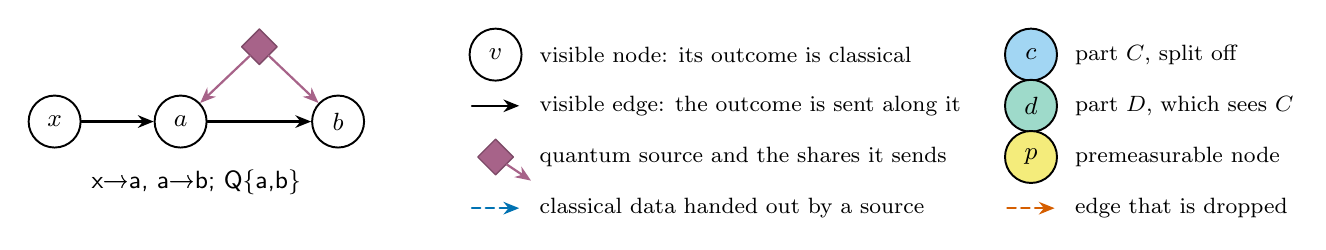
\begin{tikzpicture}[mdag]
  % a small structure
  \vn{x}{0,0}{$x$} \vn{a}{1.6,0}{$a$} \vn{b}{3.6,0}{$b$}
  \qs{q}{2.6,0.95}
  \de{x}{a} \de{a}{b} \feed{q}{a,b}
  \node[lab,anchor=north] at (1.8,-0.55) {\str{x→a, a→b; Q\{a,b\}}};
  % legend
  \begin{scope}[shift={(5.6,0.85)}]
    \vn{l1}{0,0}{$v$} \node[lab,anchor=west] at (0.5,0) {visible node: its outcome is classical};
    \draw[edge] (-0.3,-0.65) -- (0.3,-0.65); \node[lab,anchor=west] at (0.5,-0.65) {visible edge: the outcome is sent along it};
    \qs{l2}{0,-1.3} \draw[qedge] (l2) -- ++(0.45,-0.3); \node[lab,anchor=west] at (0.5,-1.3) {quantum source and the shares it sends};
    \draw[cedge] (-0.3,-1.95) -- (0.3,-1.95); \node[lab,anchor=west] at (0.5,-1.95) {classical data handed out by a source};
  \end{scope}
  \begin{scope}[shift={(12.4,0.85)}]
    \vn[Cn]{m1}{0,0}{$c$} \node[lab,anchor=west] at (0.5,0) {part $C$, split off};
    \vn[Dn]{m2}{0,-0.65}{$d$} \node[lab,anchor=west] at (0.5,-0.65) {part $D$, which sees $C$};
    \vn[pre]{m3}{0,-1.3}{$p$} \node[lab,anchor=west] at (0.5,-1.3) {premeasurable node};
    \draw[dropedge] (-0.3,-1.95) -- (0.3,-1.95); \node[lab,anchor=west] at (0.5,-1.95) {edge that is dropped};
  \end{scope}
\end{tikzpicture}
\caption{Conventions. Structures are also written in the repository's notation: the visible edges, then the
sources, \str{Q\{\dots\}} for a quantum source. An orange source is the one a rule acts on.}
\label{fig:legend}
\end{figure}

\section{Models and two proof tools}\label{sec:setting}
A structure $\G$ is an mDAG \cite{Evans}: a directed acyclic graph on visible nodes $V$, together with
independent sources. Each source is a set $F\subseteq V$ of at least two members, with no source contained in another. A node $v$ sees the
outcomes of its visible parents $\Pa(v)$, called its \emph{settings}. For example,
\str{0→1, 1→2; Q\{1,2\}} describes the instrumental scenario.

\begin{definition}[Model sets]\label{def:model}
A quantum source $F$ prepares a state $\rho_F$ on $\bigotimes_{v\in F}\Hil_{F,v}$. Each node $v$
measures all its shares jointly, with a positive operator-valued measure (POVM) selected by its settings. For an assignment $x_V$,
\begin{equation}\label{eq:trace}
P(x_V)=\Tr\!\left[\left(\bigotimes_{v\in V}M_v^{x_v\mid x_{\Pa(v)}}\right)
                           \left(\bigotimes_F\rho_F\right)\right].
\end{equation}
The distributions so obtained form $\Q(\G)$. Spaces are finite-dimensional, alphabets are finite, and
no closure is taken. Diagonal states and measurements in compatible product bases give $\C(\G)$:
each source supplies a classical latent variable, and each node samples a response using its settings
and latents. Private randomness and private states can be absorbed into the measurement.
\end{definition}
On diagonal states the trace reduces to the familiar classical factorisation
\[
 P(x_V)=\sum_{\lambda}\prod_F p_F(\lambda_F)
              \prod_v p_v(x_v\mid x_{\Pa(v)},\lambda_{F\ni v}).
\]
This makes the independence of different sources explicit. Quantumly a node receiving several
shares may measure them jointly. That freedom is used by the relay in \cref{thm:sixnode}.

Summing outcomes in reverse topological order normalises \cref{eq:trace}. Model-set equalities and
inclusions hold for every choice of visible alphabets. A \emph{QC gap} needs one choice with a
distribution in $\Q(\G)\setminus\C(\G)$. We write $\qeq$ and $\ceq$ for equality of the respective sets.

\begin{lemma}[Structural dominance]\label{lem:monotone}
If $\G'$ has the same visible nodes, uses a subset of the edges of $\G$, and each of its sources lies
inside a source of $\G$, then $\Q(\G')\subseteq\Q(\G)$ and $\C(\G')\subseteq\C(\G)$.
\end{lemma}
\begin{proof}
Assign each smaller source to a containing source. Each containing source distributes the tensor product
of its assigned states, and every node ignores extra settings. This also works for diagonal models.
\end{proof}
\begin{corollary}[Sandwich]\label{cor:sandwich}
A structure lying structurally between two equivalent structures has the same model set as both,
by the two inclusions above. This holds separately for quantum and classical models.
\end{corollary}

\begin{definition}\label{def:prem}
A \emph{premeasurable} node has one source and no visible parents.
\end{definition}

\begin{lemma}[Pre-measurement]\label{lem:premeasure}
Let $a$ be premeasurable with source $F$. Every quantum model of $\G$ can be replaced by a model of $\G$ with the
same distribution in which the share of every member of $F$ contains a classical register holding the outcome
$x_a$, and $a$ outputs its register. If the given model is classical, so is the new one.
\end{lemma}
\begin{proof}
Since $a$ has no visible parent and no other source, its POVM is a single POVM $\{M_a^{x}\}_x$ on $\Hil_{F,a}$.
Replace $\rho_F$ by
\[
\rho_F'=\sum_{x}\;\proj{x}^{\otimes F}\otimes\Tr_{\Hil_{F,a}}\bigl[(M_a^{x}\otimes\id)\,\rho_F\bigr],
\]
where $\proj{x}^{\otimes F}$ is one copy of a classical register for each member of $F$, the copy of $a$ replacing
$\Hil_{F,a}$. Node $a$ measures its register; every other member applies its old POVM to its old share and ignores
its register. For each $x_V$ the number \eqref{eq:trace} is the same as before: the factor $M_a^{x_a}$ has been
moved from the measurement into the state. If the given model is classical, $\rho_F'$ is diagonal and so is the
measurement of the register.
\end{proof}

\begin{figure}[H]
\centering
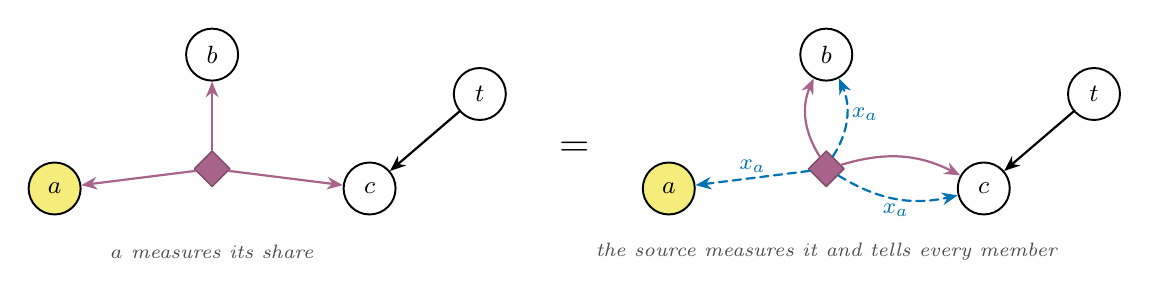
\begin{tikzpicture}[mdag]
  \begin{scope}
    \vn[pre]{a}{0,0}{$a$} \vn{b}{2.0,1.7}{$b$} \vn{c}{4.0,0}{$c$} \vn{t}{5.4,1.2}{$t$}
    \qs{q}{2.0,0.25}
    \feed{q}{a,b,c} \de{t}{c}
    \node[tag] at (2.0,-0.8) {$a$ measures its share};
  \end{scope}
  \node[rel] at (6.6,0.5) {$=$};
  \begin{scope}[shift={(7.8,0)}]
    \vn[pre]{a}{0,0}{$a$} \vn{b}{2.0,1.7}{$b$} \vn{c}{4.0,0}{$c$} \vn{t}{5.4,1.2}{$t$}
    \qs{q}{2.0,0.25}
    \draw[qedge] (q) to[bend left=28] (b); \draw[qedge] (q) to[bend left=22] (c);
    \draw[cedge] (q) -- node[lab,above,text=ccol] {$x_a$} (a);
    \draw[cedge] (q) to[bend right=28] node[lab,right,text=ccol,pos=0.55] {$x_a$} (b);
    \draw[cedge] (q) to[bend right=22] node[lab,below,text=ccol] {$x_a$} (c);
    \de{t}{c}
    \node[tag] at (2.0,-0.8) {the source measures it and tells every member};
  \end{scope}
\end{tikzpicture}
\caption{A fixed measurement can move into its source. Every member then receives a register containing the outcome, along with its conditional quantum share where needed.}
\label{fig:premeasure}
\end{figure}

\begin{ideabox}{The catalogue}
Suppose the visible value $z$ leaves a group of nodes holding a state $\tau_z$. A source serving the group
can prepare $\bigotimes_z\tau_z$ in advance. If every member learns $z$, each measures its share of the
same entry. All unused entries have trace one. This works when the steered systems have no residual
correlations with an outsider beyond $z$. Closure in \cref{thm:split} supplies precisely that guarantee.
\end{ideabox}

\begin{figure}[H]
\centering
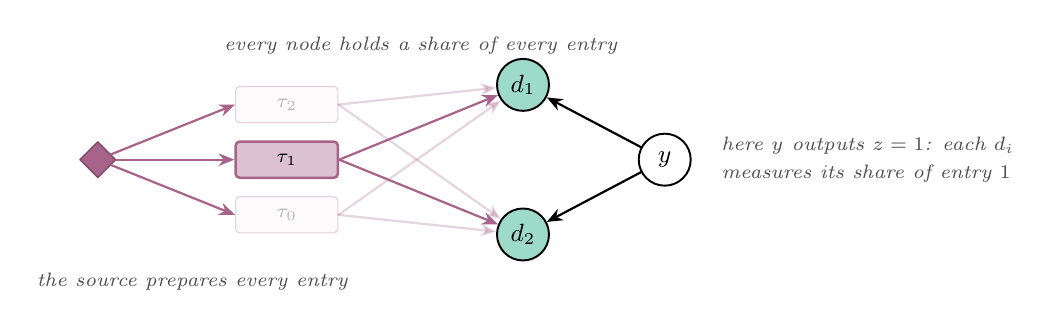
\begin{tikzpicture}[mdag]
  \tikzset{entry/.style={draw=qcol, fill=qcol!12, rounded corners=1.5pt, minimum width=13mm, minimum height=4.6mm,
                         font=\scriptsize}}
  \qs{q}{0,0.8}
  \node[entry, faint] (e0) at (2.4,0.1) {$\tau_{0}$};
  \node[entry, line width=0.9pt, fill=qcol!40] (e1) at (2.4,0.8) {$\tau_{1}$};
  \node[entry, faint] (e2) at (2.4,1.5) {$\tau_{2}$};
  \foreach \e in {e0,e1,e2} { \draw[qedge] (q) -- (\e.west); }
  \vn[Dn]{d1}{5.4,1.75}{$d_1$} \vn[Dn]{d2}{5.4,-0.15}{$d_2$} \vn{y}{7.2,0.8}{$y$}
  \foreach \e in {e0,e2} { \draw[qedge,faint] (\e.east) -- (d1); \draw[qedge,faint] (\e.east) -- (d2); }
  \draw[qedge] (e1.east) -- (d1); \draw[qedge] (e1.east) -- (d2);
  \de{y}{d1} \de{y}{d2}
  \node[tag,anchor=west] at (7.8,0.98) {here $y$ outputs $z=1$: each $d_i$};
  \node[tag,anchor=west] at (7.8,0.62) {measures its share of entry $1$};
  \node[tag] at (1.2,-0.75) {the source prepares every entry};
  \node[tag] at (4.1,2.25) {every node holds a share of every entry};
\end{tikzpicture}
\caption{The source prepares all entries. Both receivers see $z=1$ and select their shares of the same entry.}
\label{fig:catalogue}
\end{figure}


\section{Face splitting}\label{sec:split}
Think of $C$ as the part of a source whose outcomes are seen, and $D$ as the part that sees them.
If $D$ can select its steered state from a catalogue, the two parts can be supplied separately.

\begin{rulebox}{Face splitting for a closed family of sources}
\begin{theorem}\label{thm:split}
Let $D$ be a non-empty set of nodes of $\G$ and let $F_1,\dots,F_k$ $(k\ge 1)$ be distinct sources that strictly
contain $D$. Put $C_i=F_i\setminus D$ and $C=C_1\cup\dots\cup C_k$; the other sources of $\G$ are the
\emph{remaining} ones. Assume
\begin{description}[leftmargin=1.9cm,style=nextline,itemsep=1pt]
\item[(S1) closure] no remaining source contains a node of $C$ (the family $F_1,\dots,F_k$ is \emph{closed});
\item[(S2) visibility] every node of $D$ sees all nodes of $C$ and all their settings:
  $C\cup\Pa(C)\subseteq\Pa(d)$ for every $d\in D$, where $\Pa(C)=\bigcup_{c\in C}\Pa(c)$.
\end{description}
Let $\G'$ be obtained from $\G$ by replacing the sources $F_1,\dots,F_k$ by $C_1,\dots,C_k$ and $D$, and then
discarding every set that has a single member or is contained in another source. Then
\[
\Q(\G')=\Q(\G)\qquad\text{and}\qquad\C(\G')=\C(\G).
\]
\end{theorem}
\end{rulebox}

\begin{figure}[H]
\centering
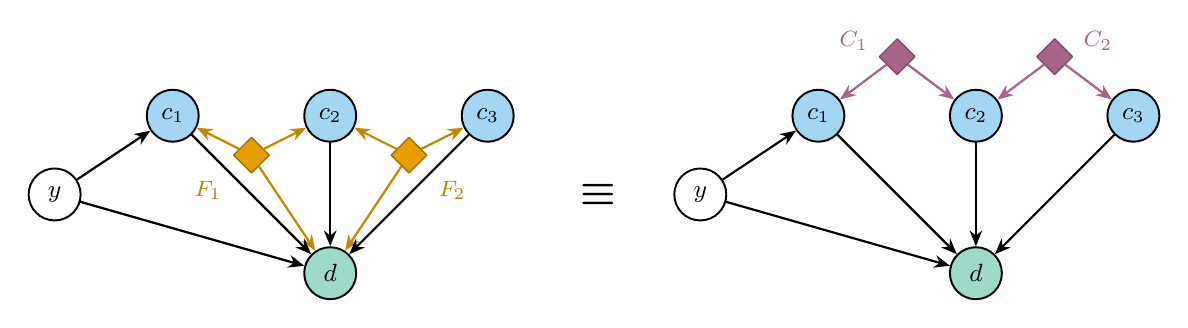
\begin{tikzpicture}[mdag]
  \begin{scope}
    \vn{y}{-1.5,1.0}{$y$}
    \vn[Cn]{c1}{0,2}{$c_1$} \vn[Cn]{c2}{2,2}{$c_2$} \vn[Cn]{c3}{4,2}{$c_3$} \vn[Dn]{d}{2,0}{$d$}
    \qs[splitsrc]{f1}{1.0,1.5} \qs[splitsrc]{f2}{3.0,1.5}
    \feed[splitedge]{f1}{c1,c2,d} \feed[splitedge]{f2}{c2,c3,d}
    \de{c1}{d} \de{c2}{d} \de{c3}{d} \de{y}{c1} \de{y}{d}
    \node[lab,text=splitcol!80!black] at (0.45,1.05) {$F_1$}; \node[lab,text=splitcol!80!black] at (3.55,1.05) {$F_2$};
  \end{scope}
  \node[rel] at (5.4,1.0) {\equivsign};
  \begin{scope}[shift={(8.2,0)}]
    \vn{y}{-1.5,1.0}{$y$}
    \vn[Cn]{c1}{0,2}{$c_1$} \vn[Cn]{c2}{2,2}{$c_2$} \vn[Cn]{c3}{4,2}{$c_3$} \vn[Dn]{d}{2,0}{$d$}
    \qs{f1}{1.0,2.75} \qs{f2}{3.0,2.75}
    \feed{f1}{c1,c2} \feed{f2}{c2,c3}
    \de{c1}{d} \de{c2}{d} \de{c3}{d} \de{y}{c1} \de{y}{d}
    \node[lab,text=qcol] at (0.45,2.95) {$C_1$}; \node[lab,text=qcol] at (3.55,2.95) {$C_2$};
  \end{scope}
\end{tikzpicture}
\caption{Two overlapping sources are split along $D=\{d\}$. The green receiver sees $c_1,c_2,c_3$ and the setting $y$. Splitting both orange sources leaves the blue nodes sharing the two smaller sources.}
\label{fig:split-generic}
\end{figure}

\begin{figure}[H]
\centering
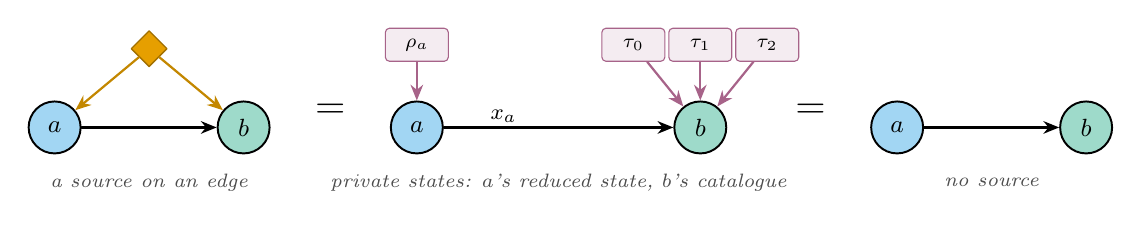
\begin{tikzpicture}[mdag]
  \begin{scope}
    \vn[Cn]{a}{0,0}{$a$} \vn[Dn]{b}{2.4,0}{$b$} \qs[splitsrc]{q}{1.2,1.0}
    \feed[splitedge]{q}{a,b} \de{a}{b}
    \node[tag] at (1.2,-0.7) {a source on an edge};
  \end{scope}
  \node[rel] at (3.5,0.2) {$=$};
  \begin{scope}[shift={(4.6,0)}]
    \vn[Cn]{a}{0,0}{$a$} \vn[Dn]{b}{3.6,0}{$b$}
    \de{a}{b} \node[lab,above] at (1.1,0) {$x_a$};
    \node[draw=qcol, fill=qcol!12, rounded corners=1.5pt, minimum width=8mm, minimum height=4.2mm, font=\scriptsize] (r) at (0,1.05) {$\rho_a$};
    \draw[qedge] (r) -- (a);
    \foreach \i/\lbl in {0/{$\tau_{0}$},1/{$\tau_{1}$},2/{$\tau_{2}$}} {
      \node[draw=qcol, fill=qcol!12, rounded corners=1.5pt, minimum width=8mm, minimum height=4.2mm, font=\scriptsize]
        (e\i) at ({2.75+0.85*\i},1.05) {\lbl};
      \draw[qedge] (e\i) -- (b);
    }
    \node[tag] at (1.8,-0.7) {private states: $a$'s reduced state, $b$'s catalogue};
  \end{scope}
  \node[rel] at (9.6,0.2) {$=$};
  \begin{scope}[shift={(10.7,0)}]
    \vn[Cn]{a}{0,0}{$a$} \vn[Dn]{b}{2.4,0}{$b$} \de{a}{b}
    \node[tag] at (1.2,-0.7) {no source};
  \end{scope}
\end{tikzpicture}
\caption{The smallest case of \cref{thm:split}: $C=\{a\}$, $D=\{b\}$, $k=1$. The entry $\tau_x$ of the catalogue is
the state that the outcome $x$ of $a$ would have left on the share of $b$.}
\label{fig:split-idea}
\end{figure}

With just $a\to b$ and the source $\{a,b\}$, measuring $a$ leaves $b$ a state determined by $x_a$.
The edge tells $b$ which state to prepare locally. For several receivers this private preparation becomes
a shared catalogue. If $a$ also has a setting, every receiver needs that setting to select its entry.

\begin{proof}[Proof of \cref{thm:split}]
Structural dominance gives one inclusion. For the other, fix a model of the unsplit family and put
$Y=\Pa(C)\setminus C$, $z=(x_C,x_Y)$. By (S1) the product $M_C(z)$ of the measurements at $C$
acts only on shares of the $F_i$. After tracing out those shares, the operator left on $D$ is
\[
 \tau_z=\Tr_C\!\left[(M_C(z)\otimes\id)\bigotimes_i\rho_{F_i}\right],
 \qquad q_z=\Tr\tau_z.
\]
The trace $q_z$ is also the weight of $x_C$ at those settings when each $C_i$ receives its own reduced
state $\Tr_D\rho_{F_i}$. Supply these reduced states independently and keep the old measurements at $C$.
Let the new source on $D$ emit a catalogue with entry $\tau_z/q_z$ whenever $q_z>0$, and a fixed state
otherwise. By (S2) each $d\in D$ reads $z$ and measures the matching entry together with its other shares.
A singleton can prepare its entry privately, and a source containing $D$ can distribute the catalogue.

For each assignment in \cref{eq:trace}, the weight $q_z$ times the selected state gives exactly $\tau_z$.
Zero weight contributes zero in both models. Everything outside the family sees the same visible values
and retains its old shares. Diagonal inputs give diagonal entries, proving the classical equality too.
\end{proof}

\begin{validbox}[label=ex:setting]{a setting that both nodes see}
\begin{minipage}{0.55\linewidth}
$D=\{d\}$, $F_1=\{c,d\}$, $C=\{c\}$, and $c$ has a setting $y$. (S2) asks that $d$ see $y$ as well, which
holds:\\[3pt]
\str{y→c, y→d, c→d; Q\{c,d\}} \ $\equiv$ \ \str{y→c, y→d, c→d}.\\[3pt]
The catalogue is indexed by $(x_c,x_y)$. The edge $y\to d$ supplies the second index.
\end{minipage}\hfill
\begin{minipage}{0.42\linewidth}\centering
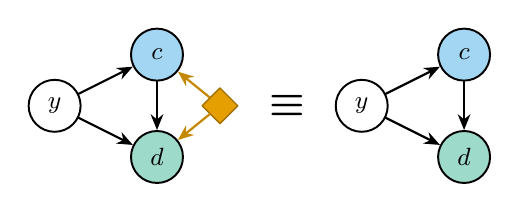
\begin{tikzpicture}[mdag]
  \vn{y}{0,0.65}{$y$} \vn[Cn]{c}{1.3,1.3}{$c$} \vn[Dn]{d}{1.3,0}{$d$} \qs[splitsrc]{q}{2.1,0.65}
  \feed[splitedge]{q}{c,d} \de{y}{c} \de{y}{d} \de{c}{d}
  \node[rel] at (2.95,0.65) {\equivsign};
  \begin{scope}[shift={(3.9,0)}]
    \vn{y}{0,0.65}{$y$} \vn[Cn]{c}{1.3,1.3}{$c$} \vn[Dn]{d}{1.3,0}{$d$}
    \de{y}{c} \de{y}{d} \de{c}{d}
  \end{scope}
\end{tikzpicture}
\end{minipage}
\end{validbox}

\begin{validbox}[label=ex:together]{two sources that must be split together}
\begin{minipage}{0.5\linewidth}
$D=\{d\}$, $F_1=\{a,b,d\}$, $F_2=\{a,c,d\}$, so $C_1=\{a,b\}$ and $C_2=\{a,c\}$ have the node $a$ in common, which
is also a parent of $b$ and $c$.\\[3pt]
\str{a→b, a→c, a→d, b→d, c→d; Q\{a,b,d\}, Q\{a,c,d\}} \ $\equiv$\\
\str{a→b, a→c, a→d, b→d, c→d; Q\{a,b\}, Q\{a,c\}}.\\[3pt]
Here $a$ may measure its two shares jointly. Once $a$, $b$ and $c$ have all measured, their outcomes determine
an entry of the catalogue on the two shares of $d$. Neither source satisfies (S1) on its own, and
with $k=1$ alone the two structures stay in different classes.
\end{minipage}\hfill
\begin{minipage}{0.47\linewidth}\centering
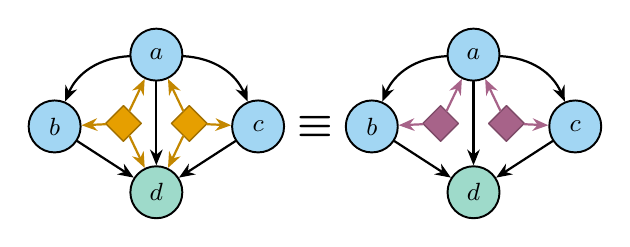
\begin{tikzpicture}[mdag,scale=0.76]
  \newcommand{\togethernodes}{\vn[Cn]{a}{1.5,2.3}{$a$} \vn[Cn]{b}{-0.2,1.1}{$b$} \vn[Cn]{c}{3.2,1.1}{$c$}
    \vn[Dn]{d}{1.5,0}{$d$} \de{a}{d} \de{b}{d} \de{c}{d}
    \draw[edge] (a) to[bend right=32] (b); \draw[edge] (a) to[bend left=32] (c);}
  \togethernodes
  \qs[splitsrc]{f1}{0.95,1.15} \qs[splitsrc]{f2}{2.05,1.15}
  \feed[splitedge]{f1}{a,b,d} \feed[splitedge]{f2}{a,c,d}
  \node[rel] at (4.15,1.1) {\equivsign};
  \begin{scope}[shift={(5.3,0)}]
    \togethernodes
    \qs{f1}{0.95,1.15} \qs{f2}{2.05,1.15}
    \feed{f1}{a,b} \feed{f2}{a,c}
  \end{scope}
\end{tikzpicture}
\end{minipage}
\end{validbox}

\paragraph{Comparison with classical face splitting.}
The classical rules of Ansanelli, Wolfe and Spekkens \cite{AWS} share the visibility condition (S2).
They differ in which other sources may meet $C$. The last column gives the number of four-node classes
if that splitting rule is used alongside the quantum edge rules.

\begin{center}\small
\begin{tabular}{@{}lp{8cm}cr@{}}
\toprule
Splitting rule & Other sources allowed to meet $C$ & Quantum valid & Classes\\
\midrule
Weak & None for each individual split & yes & 461\\
Closed family & Other sources split along with it & yes & 446\\
Moderate & Remaining sources that contain $D$ & no & 450\\
Strong & Both kinds & no & 438\\
\bottomrule
\end{tabular}
\end{center}
The joint split above goes beyond the weak rule. The six-node witness in \cref{sec:leaky} rules out
moderate splitting in general, including as a special case of the strong rule. For a fixed $D$ the
code need only split the largest closed family satisfying (S2). Splitting fewer sources gives an
intermediate structure covered by the sandwich (\cref{cor:sandwich}).

\section{Edge dropping}\label{sec:edge}
The classical edge rule of Henson, Lal and Pusey \cite{HLP,Evans,AWS} removes $a\to b$ under two hypotheses:
\begin{description}[leftmargin=1.2cm]
\item[(H1)] $a$ belongs to at least one source, and every source of $a$ also contains $b$.
\item[(H2)] $b$ sees every visible parent of $a$.
\end{description}
Classically, $b$ can compute $a$'s response from its settings, latents and private noise (a shared
latent can supply that noise). A quantum share generally cannot predict the measurement on another
share. Rules A and B give two ways for the target to recover the missing outcome.

\begin{figure}[H]
\centering
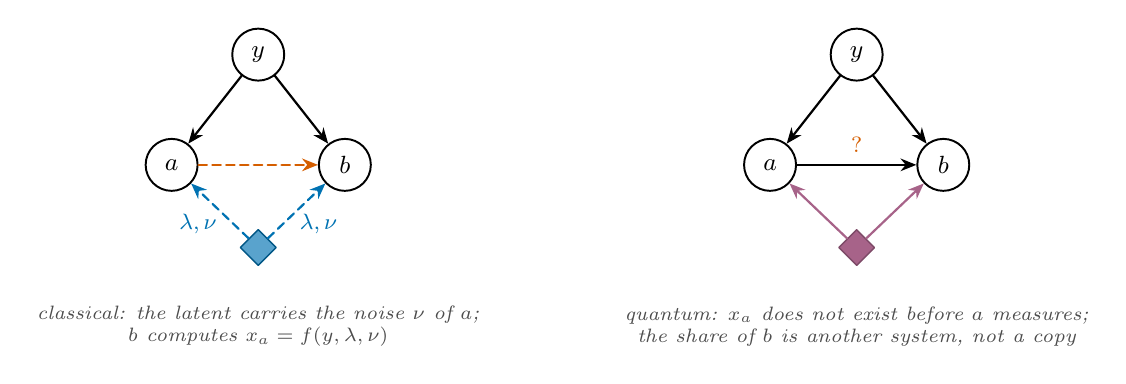
\begin{tikzpicture}[mdag]
  \begin{scope}
    \vn{y}{1.1,1.7}{$y$} \vn{a}{0,0.3}{$a$} \vn{b}{2.2,0.3}{$b$} \qs[csrc]{q}{1.1,-0.75}
    \draw[cedge] (q) -- node[lab,below left=-1pt,text=ccol] {$\lambda,\nu$} (a);
    \draw[cedge] (q) -- node[lab,below right=-1pt,text=ccol] {$\lambda,\nu$} (b);
    \de{y}{a} \de{y}{b} \de[dropedge]{a}{b}
    \node[tag,align=center] at (1.1,-1.75) {classical: the latent carries the noise $\nu$ of $a$;\\
      $b$ computes $x_a=f(y,\lambda,\nu)$};
  \end{scope}
  \begin{scope}[shift={(7.6,0)}]
    \vn{y}{1.1,1.7}{$y$} \vn{a}{0,0.3}{$a$} \vn{b}{2.2,0.3}{$b$} \qs{q}{1.1,-0.75}
    \feed{q}{a,b} \de{y}{a} \de{y}{b} \de{a}{b}
    \node[lab,text=dropcol] at (1.1,0.55) {?};
    \node[tag,align=center] at (1.1,-1.75) {quantum: $x_a$ does not exist before $a$ measures;\\
      the share of $b$ is another system, not a copy};
  \end{scope}
\end{tikzpicture}
\caption{Why the classical argument for dropping $a\to b$ has no quantum counterpart. On the left the source is
classical (blue) and hands $a$ and $b$ the same data.}
\label{fig:edge-idea}
\end{figure}

\subsection{Rule A: the origin and its settings}

\begin{rulebox}{Edge dropping, Rule A}
\begin{theorem}[Rule A: the origin is premeasurable]\label{thm:ruleA}
Let the edge $a\to b$ satisfy (H1) and (H2), and let $a$ be premeasurable. Then
\[\Q(\G)=\Q(\G-(a\to b))\qquad\text{and}\qquad\C(\G)=\C(\G-(a\to b)).\]
\end{theorem}
\end{rulebox}

\begin{proof}
By \cref{lem:premeasure}, $b$ can read $x_a$ from the shared source and select its old measurement.
Adding the edge back is structural dominance. Both constructions preserve diagonal models.
\end{proof}

\begin{figure}[H]
\centering
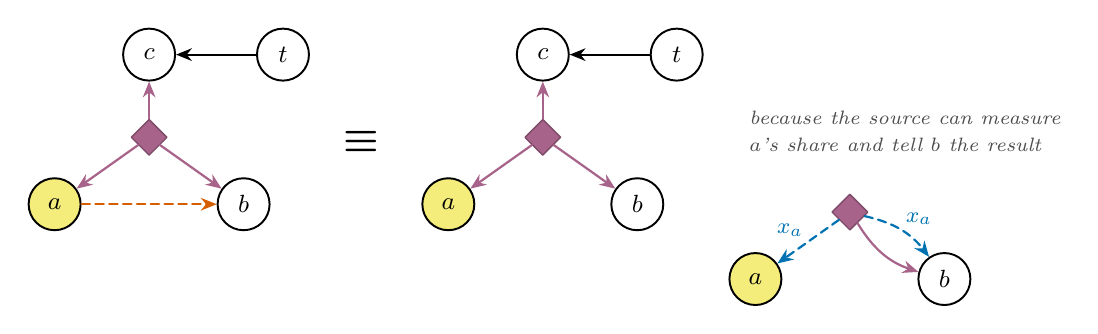
\begin{tikzpicture}[mdag]
  \begin{scope}
    \vn[pre]{a}{0,0}{$a$} \vn{b}{2.4,0}{$b$} \vn{c}{1.2,1.9}{$c$} \vn{t}{2.9,1.9}{$t$}
    \qs{q}{1.2,0.85}
    \feed{q}{a,b,c} \de[dropedge]{a}{b} \de{t}{c}
  \end{scope}
  \node[rel] at (3.9,0.8) {\equivsign};
  \begin{scope}[shift={(5.0,0)}]
    \vn[pre]{a}{0,0}{$a$} \vn{b}{2.4,0}{$b$} \vn{c}{1.2,1.9}{$c$} \vn{t}{2.9,1.9}{$t$}
    \qs{q}{1.2,0.85}
    \feed{q}{a,b,c} \de{t}{c}
  \end{scope}
  \node[tag,anchor=west] at (8.7,1.1) {because the source can measure};
  \node[tag,anchor=west] at (8.7,0.75) {$a$'s share and tell $b$ the result};
  \begin{scope}[shift={(8.9,-0.95)}]
    \vn[pre]{a}{0,0}{$a$} \vn{b}{2.4,0}{$b$} \qs{q}{1.2,0.85}
    \draw[cedge] (q) -- node[lab,above left,text=ccol] {$x_a$} (a);
    \draw[cedge] (q) to[bend left=20] node[lab,above right,text=ccol,pos=0.5] {$x_a$} (b);
    \draw[qedge] (q) to[bend right=20] (b);
  \end{scope}
\end{tikzpicture}
\caption{Rule A. The yellow origin has no setting and a single source, which also contains the target. The
bystander $c$ is arbitrary; here it has a setting.}
\label{fig:ruleA}
\end{figure}

\begin{proposition}[Rule A with settings that every member sees]\label{prop:ruleA-settings}
Let the edge $a\to b$ satisfy (H1), let $a$ be a member of exactly one source $F$, and let every setting of $a$ be
a setting of every other member of $F$. Then $\Q(\G)=\Q(\G-(a\to b))$ and $\C(\G)=\C(\G-(a\to b))$.
\end{proposition}

\begin{proof}
For every setting $y$ the sole source $F$ prepares an independent entry
\[
 \omega_y=\sum_x\proj{x}_{R_a}\otimes\proj{x}_{R_b}\otimes
          \Tr_{F,a}\!\left[(M_a^{x\mid y}\otimes\id)\rho_F\right].
\]
All members know $y$. In that entry $a$ outputs its register and $b$ uses its copy to select its
old measurement. Every other member measures its share as before. The selected term in \cref{eq:trace}
is the original one and the unused entries have trace one. Diagonal models stay diagonal.
\end{proof}

\begin{validbox}[label=ex:target-two]{Rule A; the target may have further sources}
\begin{minipage}{0.55\linewidth}
The origin $0$ is premeasurable with the source $\{0,1\}$. The target $1$ is also a member of $\{1,2\}$ and may
measure its two shares jointly; Rule A does not mind:\\[3pt]
\str{0→1; Q\{0,1\}, Q\{1,2\}} \ $\equiv$ \ \str{Q\{0,1\}, Q\{1,2\}}.\\[3pt]
The reverse move adds an edge from a premeasurable setting in \cref{fig:bell-class}.
\end{minipage}\hfill
\begin{minipage}{0.42\linewidth}\centering
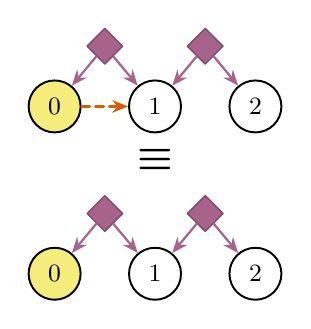
\begin{tikzpicture}[mdag,scale=0.85]
  \newcommand{\chainnodes}{\vn[pre]{a}{0,0}{$0$} \vn{b}{1.5,0}{$1$} \vn{c}{3.0,0}{$2$}
    \qs{q}{0.75,0.9} \qs{r}{2.25,0.9} \feed{q}{a,b} \feed{r}{b,c}}
  \chainnodes \de[dropedge]{a}{b}
  \node[rel] at (1.5,-0.8) {\equivsign};
  \begin{scope}[shift={(0,-2.5)}] \chainnodes \end{scope}
\end{tikzpicture}
\end{minipage}
\end{validbox}

\subsection{Rule B: the bystanders}
The bystanders are the members other than $a,b$ of the sources containing $a$. The origin can now
have several sources and its measurements can depend on settings.

\begin{rulebox}{Edge dropping, Rule B}
\begin{theorem}[Rule B: every bystander is premeasurable]\label{thm:ruleB}
Let the edge $a\to b$ satisfy (H1) and (H2), and let every bystander be premeasurable. Then
\[\Q(\G)=\Q(\G-(a\to b))\qquad\text{and}\qquad\C(\G)=\C(\G-(a\to b)).\]
\end{theorem}
\end{rulebox}

\begin{figure}[H]
\centering
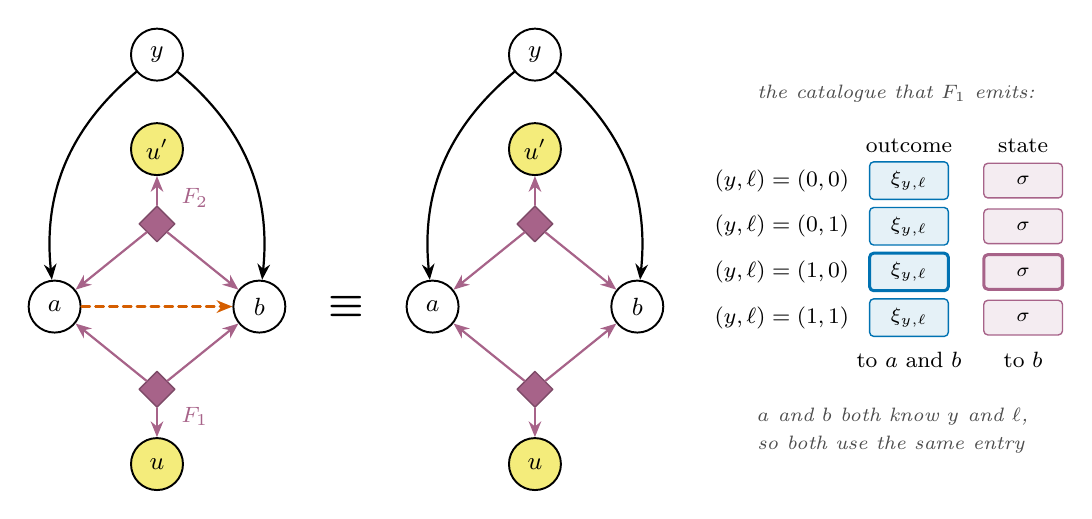
\begin{tikzpicture}[mdag]
  \newcommand{\ruleBnodes}{\vn{y}{1.3,4.2}{$y$} \vn{a}{0,1.0}{$a$} \vn{b}{2.6,1.0}{$b$}
    \vn[pre]{u}{1.3,-1.0}{$u$} \vn[pre]{up}{1.3,3.0}{$u'$}
    \qs{f1}{1.3,-0.05} \qs{f2}{1.3,2.05}
    \feed{f1}{a,b,u} \feed{f2}{a,b,up}
    \draw[edge] (y) to[bend right=28] (a); \draw[edge] (y) to[bend left=28] (b);}
  \begin{scope}
    \ruleBnodes \de[dropedge]{a}{b}
    \node[lab,text=qcol] at (1.78,-0.4) {$F_1$}; \node[lab,text=qcol] at (1.78,2.38) {$F_2$};
  \end{scope}
  \node[rel] at (3.7,1.0) {\equivsign};
  \begin{scope}[shift={(4.8,0)}]
    \ruleBnodes
  \end{scope}
  \begin{scope}[shift={(9.1,0.7)}]
    \tikzset{cell/.style={rounded corners=1.5pt, minimum width=10mm, minimum height=4.4mm, font=\scriptsize}}
    \node[tag,anchor=west] at (-0.3,3.0) {the catalogue that $F_1$ emits:};
    \node[lab,anchor=south] at (1.75,2.2) {outcome}; \node[lab,anchor=south] at (3.2,2.2) {state};
    \foreach \j/\lbl/\w in {0/{$(y,\ell)=(0,0)$}/0.5pt, 1/{$(y,\ell)=(0,1)$}/0.5pt, 2/{$(y,\ell)=(1,0)$}/1.1pt, 3/{$(y,\ell)=(1,1)$}/0.5pt} {
      \node[lab,anchor=east] at (1.05,{1.9-0.58*\j}) {\lbl};
      \node[cell, draw=ccol, fill=ccol!10, line width=\w] at (1.75,{1.9-0.58*\j}) {$\xi_{y,\ell}$};
      \node[cell, draw=qcol, fill=qcol!12, line width=\w] at (3.2,{1.9-0.58*\j}) {$\sigma$};
    }
    \node[lab,anchor=north] at (1.75,-0.22) {to $a$ and $b$}; \node[lab,anchor=north] at (3.2,-0.22) {to $b$};
    \node[tag,anchor=west] at (-0.3,-1.1) {$a$ and $b$ both know $y$ and $\ell$,};
    \node[tag,anchor=west] at (-0.3,-1.45) {so both use the same entry};
  \end{scope}
\end{tikzpicture}
\caption{Rule B. The origin $a$ has a setting $y$, which $b$ also sees, and two sources, both of which contain
$b$. The bystanders $u$ and $u'$ are premeasurable; $\ell$ stands for their outcomes.}
\label{fig:ruleB}
\end{figure}

\begin{proof}
Write $F_i$ for the sources of $a$ and $U_i=F_i\setminus\{a,b\}$. Pre-measure each bystander.
Source $F_i$ draws its bystander outcomes $\ell_i$ and shares them with its members. Before measuring
$a$, these draws are independent across sources, with joint weight $p(\ell)=\prod_i p_i(\ell_i)$.
For fixed $\ell$ and origin settings $y$, measuring $a$ on all its shares gives a distribution
$r(x\mid y,\ell)$ and a conditional state $\sigma_{x,y,\ell}$ on $b$'s shares of the $F_i$.
These are the only systems left in those sources. In the original model their unnormalised state is
\[
 \tau(x;y,\ell)=\Tr_{a,U}\!\left[
  \left(M_a^{x\mid y}\otimes\bigotimes_{u\in U}M_u^{\ell_u}\otimes\id_b\right)
  \bigotimes_i\rho_{F_i}\right]
 =p(\ell)r(x\mid y,\ell)\sigma_{x,y,\ell},
\]
where $U=\bigcup_i U_i$ and the trace is over the shares held by $a$ and $U$.
For a zero-weight entry one may choose any fixed state.

Have one shared source prepare a catalogue indexed by every $(y,\ell)$, independently of the draws.
In each entry it samples $x$ from $r$, gives $a,b$ a copy of $x$, and gives $b$ the state
$\sigma_{x,y,\ell}$. Both nodes see all the $\ell_i$ by (H1), and both see $y$ by (H2).
Node $a$ outputs the selected $x$; $b$ uses it to measure the selected state jointly with its other shares.
For each visible assignment the weight $p(\ell)r(x\mid y,\ell)$ times the conditional state recovers
the original unnormalised state at $b$. Thus \cref{eq:trace} agrees, including on zero-weight assignments.
The same construction is classical for diagonal inputs, and the reverse inclusion is structural dominance.
\end{proof}

\begin{validbox}[label=ex:ruleB-bystander]{Rule B; a premeasurable bystander}
\begin{minipage}{0.55\linewidth}
The origin $1$ has the setting $0$, seen by the target $2$; the source $\{1,2,3\}$ has the bystander $3$, which has
no setting and no other source:\\[3pt]
\str{0→1, 0→2, 1→2; Q\{1,2,3\}} \ $\equiv$ \ \str{0→1, 0→2; Q\{1,2,3\}}.\\[3pt]
Giving $3$ the setting $0$ makes every other member of the source see the origin's settings. The wider Rule A
then drops the edge (\cref{prop:ruleA-settings}), while the setting at $3$ rules out Rule B.
\end{minipage}\hfill
\begin{minipage}{0.42\linewidth}\centering
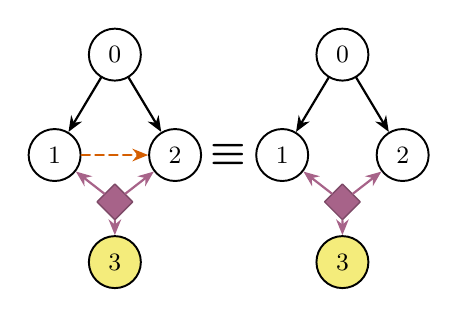
\begin{tikzpicture}[mdag,scale=0.85]
  \vn{y}{0.9,1.5}{$0$} \vn{a}{0,0}{$1$} \vn{b}{1.8,0}{$2$} \vn[pre]{o}{0.9,-1.6}{$3$} \qs{q}{0.9,-0.7}
  \feed{q}{a,b,o} \de{y}{a} \de{y}{b} \de[dropedge]{a}{b}
  \node[rel] at (2.6,0.0) {\equivsign};
  \begin{scope}[shift={(3.4,0)}]
    \vn{y}{0.9,1.5}{$0$} \vn{a}{0,0}{$1$} \vn{b}{1.8,0}{$2$} \vn[pre]{o}{0.9,-1.6}{$3$} \qs{q}{0.9,-0.7}
    \feed{q}{a,b,o} \de{y}{a} \de{y}{b}
  \end{scope}
\end{tikzpicture}
\end{minipage}
\end{validbox}

\paragraph{Using the rules together.}\label{sec:compose}
A premeasurable $p$ can send its outcome along a new edge to each other member of its sole source $F$
by Rule A. Face splitting with $C=\{p\}$ then replaces $F$ with $F\setminus\{p\}$.
The Bell examples use this exchange in both directions.

For example, add the edges from $p$ to the other members of $\{p,c,d\}$. Now $c,d$ both know $x_p$
and the source reduces to $\{c,d\}$. If a remaining source already contains $c,d$, it can carry
their catalogue. The visible arrows from $p$ still carry its outcome.

\begin{lemma}\label{lem:simultaneous}
Let $\Delta$ be the set of edges of $\G$ that satisfy Rule A with shared settings (\cref{prop:ruleA-settings})
or Rule B (\cref{thm:ruleB}) in $\G$. Then
$\G-\Delta\qeq\G$ and $\G-\Delta\ceq\G$.
\end{lemma}
\begin{proof}
Fix a topological order of $\G$ and remove the edges $(a,b)\in\Delta$ one at a time, those with a later origin $a$
first. Sources stay fixed, so (H1) persists. Removing edges also preserves the premeasurability of every
bystander in Rule B. Let $y$ be any remaining setting of $a$ when $a\to b$ is removed. For (H2) the original
graph contains $y\to b$. For Rule A it also contains $y\to v$ for every other member $v$ of the sole source of
$a$. All these edges are still present because their origin $y$ precedes $a$ in the topological order.
\end{proof}

Widening Rule A to shared settings licenses $35$ additional four-node edge deletions within known
classes. On five nodes it joins $542$ classes, reducing the count from $596{,}413$ to $595{,}871$.

\clearpage
\section{Where classical equivalences fail}\label{sec:notquantum}
Classical edge dropping and moderate face splitting can preserve $\C$ while shrinking $\Q$.
In each witness an outside party holds a quantum system correlated with the proposed replacement.
We write $a$ for the outcome of $A$, and similarly for the other parties.

\subsection{The classical edge rule}\label{sec:hlp-fails}

\Needspace{13\baselineskip}
\begin{lemma}[A party with a double is local]\label{lem:predict}
Let $Q(a,a',c\mid s,s',t)$ be a box for three parties $A$, $A'$, $C$, with inputs $s,s'\in\{0,1\}$ and $t$, that is
no-signalling: the joint distribution of the outcomes of any two parties does not depend on the input of the
third. Suppose that $A'$ behaves towards $C$ exactly as $A$ does: for $i\in\{0,1\}$ and all $\alpha,c,t$,
\[Q(a'=\alpha,\,c\mid s'=i,\,t)\;=\;Q(a=\alpha,\,c\mid s=i,\,t)\;=:\;P(\alpha,c\mid i,t).\]
Then $P$ is local: there are a distribution $\nu(a_0,a_1)$ and response functions $P(c\mid t,a_0,a_1)$ with
\[
P(a,c\mid s,t)=\sum_{a_0,a_1}\nu(a_0,a_1)\,\delta_{a,a_s}\,P(c\mid t,a_0,a_1).
\]
In particular $P$ satisfies the CHSH inequality.
\end{lemma}
\begin{proof}
Put $\mu_t(a_0,a_1,c)=Q(a=a_0,\,a'=a_1,\,c\mid s=0,\,s'=1,\,t)$. Its marginal over $a_1$ is $P(a_0,c\mid0,t)$, by
no-signalling from $A'$. Its marginal over $a_0$ is $Q(a'=a_1,c\mid s'=1,t)=P(a_1,c\mid1,t)$, by no-signalling
from $A$ and the hypothesis. Its marginal over $c$ is a distribution $\nu(a_0,a_1)$ that does not depend on $t$,
by no-signalling from $C$. So $\lambda=(a_0,a_1)$, drawn from $\nu$, with $A$ answering $a_s$ and $C$ answering
according to $\mu_t(\lambda,c)/\nu(\lambda)$ (arbitrary where $\nu(\lambda)=0$), reproduces $P$.
\end{proof}

\begin{cexbox}{the edge rule, with settings}
\begin{theorem}\label{thm:hlp-settings}
Let $\G^{+}$ have the nodes $A,B,C,S,T$, the edges $S\to A$, $S\to B$, $T\to C$, $A\to B$ and the source
$\{A,B,C\}$, and let $\G^{-}=\G^{+}-(A\to B)$. Then
\[
\C(\G^{-})=\C(\G^{+})\qquad\text{but}\qquad\Q(\G^{-})\subsetneq\Q(\G^{+}).
\]
\end{theorem}
\end{cexbox}

\begin{figure}[H]
\centering
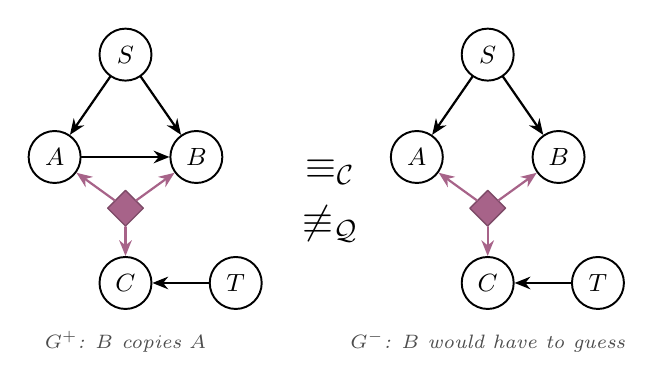
\begin{tikzpicture}[mdag]
  \begin{scope}
    \vn{s}{0.9,1.9}{$S$} \vn{a}{0,0.6}{$A$} \vn{b}{1.8,0.6}{$B$} \vn{c}{0.9,-1.0}{$C$} \vn{t}{2.3,-1.0}{$T$}
    \qs{q}{0.9,-0.05}
    \feed{q}{a,b,c} \de{s}{a} \de{s}{b} \de{t}{c} \de{a}{b}
    \node[tag] at (0.9,-1.75) {$\G^{+}$: $B$ copies $A$};
  \end{scope}
  \node[rel] at (3.5,0.4) {$\ceq$};
  \node[rel] at (3.5,-0.25) {$\not\qeq$};
  \begin{scope}[shift={(4.6,0)}]
    \vn{s}{0.9,1.9}{$S$} \vn{a}{0,0.6}{$A$} \vn{b}{1.8,0.6}{$B$} \vn{c}{0.9,-1.0}{$C$} \vn{t}{2.3,-1.0}{$T$}
    \qs{q}{0.9,-0.05}
    \feed{q}{a,b,c} \de{s}{a} \de{s}{b} \de{t}{c}
    \node[tag] at (0.9,-1.75) {$\G^{-}$: $B$ would have to guess};
  \end{scope}
\end{tikzpicture}
\caption{With $A\to B$, $B$ can copy Alice while Alice and Charlie play CHSH. Without the edge, a successful copy would supply a second Alice.}
\label{fig:hlp-settings}
\end{figure}

\begin{proof}[Proof of \cref{thm:hlp-settings}]
(H1) and (H2) give classical equality. With the edge, give $A,C$ a Bell pair, play the Clauser--Horne--Shimony--Holt (CHSH) game at independent
uniform settings $s,t$, and let $B$ copy $a$. Without the edge, $A,B,C$ would perform local measurements
on a shared state. Give $B$ its own input $s'$ to select the same measurement it would perform at $s=s'$.
The resulting box is no-signalling. When $s=s'$ we have $b=a$, so by no-signalling the $BC$ marginal
at $s'=i$ equals the $AC$ marginal at $s=i$ for either $i$. \Cref{lem:predict} makes $AC$ local,
contradicting the observed CHSH value $2\sqrt2$. Structural dominance gives the other inclusion.
\end{proof}

\begin{cexbox}{the edge rule, on four nodes without settings}
\begin{theorem}\label{thm:hlp-four}
Let $\G^{+}$ have the nodes $A,B,C,S$, the sources $\{A,B,C\}$, $\{A,B,S\}$, $\{C,S\}$ and the single edge
$A\to B$, and let $\G^{-}$ be the same without the edge. Then $\C(\G^{-})=\C(\G^{+})$ but
$\Q(\G^{-})\subsetneq\Q(\G^{+})$.
\end{theorem}
\end{cexbox}

\emph{The distribution.} $P^{*}$ is Fritz's distribution for the triangle \cite{Fritz}, with $B$ copying $A$. The
source $\{A,B,C\}$ gives $A$ and $C$ a Bell pair; $\{A,B,S\}$ gives $A$ and $S$ a uniform bit $x$; $\{C,S\}$ gives
$C$ and $S$ a uniform bit $y$. $A$ measures with the CHSH setting $x$ and outputs $(a,x)$; $C$ measures with the
setting $y$ and outputs $(c,y)$; $S$ outputs $(x,y)$; $B$ outputs what $A$ outputs. Then
$P^{*}(a,x,c,y)=\tfrac14P_{\mathrm{CHSH}}(a,c\mid x,y)$ with CHSH value $2\sqrt2$, and $P^{*}\in\Q(\G^{+})$.

\begin{figure}[H]
\centering
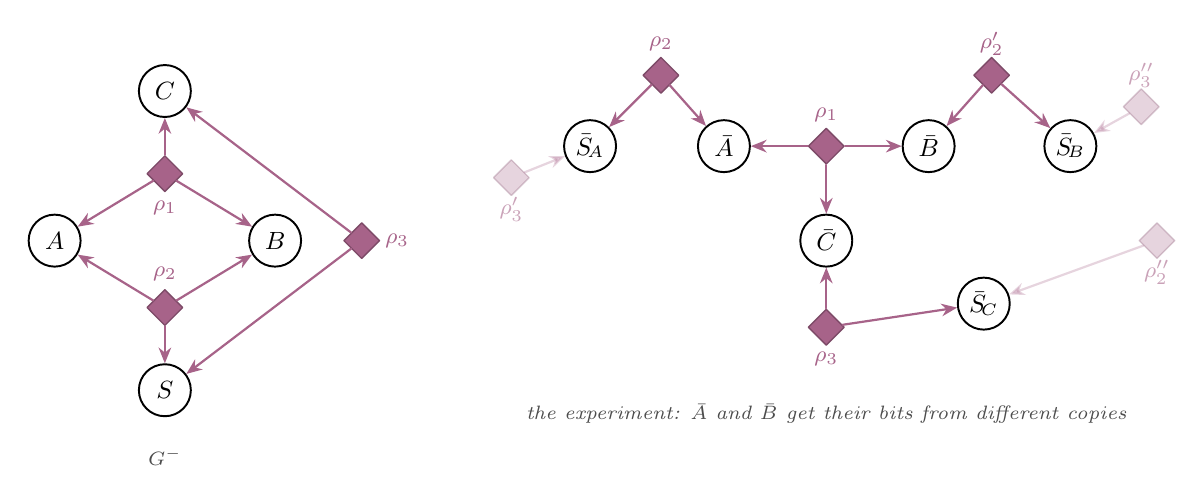
\begin{tikzpicture}[mdag]
  \begin{scope}[shift={(0,0.1)}]
    \vn{a}{0,0}{$A$} \vn{b}{2.8,0}{$B$} \vn{c}{1.4,1.9}{$C$} \vn{s}{1.4,-1.9}{$S$}
    \qs{f1}{1.4,0.85} \qs{f2}{1.4,-0.85} \qs{f3}{3.9,0}
    \feed{f1}{a,b,c} \feed{f2}{a,b,s} \feed{f3}{c,s}
    \node[lab,text=qcol] at (1.4,0.42) {$\rho_1$}; \node[lab,text=qcol] at (1.4,-0.42) {$\rho_2$};
    \node[lab,text=qcol] at (4.35,0) {$\rho_3$};
    \node[tag] at (1.4,-2.75) {$\G^{-}$};
  \end{scope}
  \begin{scope}[shift={(7.4,0.3)}]
    % sources of the experiment
    \qs{r1}{2.4,1.0}
    \qs{r2}{0.3,1.9} \qs{r2p}{4.5,1.9} \qs[src,faint]{r2pp}{6.6,-0.2}
    \qs{r3}{2.4,-1.3} \qs[src,faint]{r3p}{-1.6,0.6} \qs[src,faint]{r3pp}{6.4,1.5}
    \vn{A}{1.1,1.0}{$\bar A$} \vn{B}{3.7,1.0}{$\bar B$} \vn{C}{2.4,-0.2}{$\bar C$}
    \vn{SA}{-0.6,1.0}{$\bar S_{\!A}$} \vn{SB}{5.5,1.0}{$\bar S_{\!B}$} \vn{SC}{4.4,-1.0}{$\bar S_{\!C}$}
    \feed{r1}{A,B,C} \feed{r2}{A,SA} \feed{r2p}{B,SB} \feed{r3}{C,SC}
    \draw[qedge,faint] (r3p) -- (SA); \draw[qedge,faint] (r3pp) -- (SB); \draw[qedge,faint] (r2pp) -- (SC);
    \node[lab,text=qcol] at (2.4,1.4) {$\rho_1$}; \node[lab,text=qcol] at (0.3,2.3) {$\rho_2$};
    \node[lab,text=qcol] at (4.5,2.3) {$\rho_2'$}; \node[lab,text=qcol] at (2.4,-1.7) {$\rho_3$};
    \node[lab,text=qcol!60] at (-1.6,0.2) {$\rho_3'$}; \node[lab,text=qcol!60] at (6.4,1.9) {$\rho_3''$};
    \node[lab,text=qcol!60] at (6.6,-0.6) {$\rho_2''$};
    \node[tag] at (2.4,-2.4) {the experiment: $\bar A$ and $\bar B$ get their bits from different copies};
  \end{scope}
\end{tikzpicture}
\caption{The four-node witness and its inflation. Giving $\bar B$ a fresh copy of the setting source
preserves its correlations with $C$ while separating its setting from $A$'s.}
\label{fig:inflation}
\end{figure}

\begin{proof}
\emph{Classical.} This is the classical edge rule again: $A$ has no setting, and both its sources contain $B$.

\emph{Quantum.} $P^{*}\in\Q(\G^{+})$ as described. Suppose a quantum model of $\G^{-}$ produces $P^{*}$: states
$\rho_1$ on the shares $A_1B_1C_1$, $\rho_2$ on $A_2B_2S_2$, $\rho_3$ on $C_3S_3$, and POVMs $M_A$ (on $A_1A_2$),
$M_B$ (on $B_1B_2$), $M_C$ (on $C_1C_3$), $M_S$ (on $S_2S_3$). Consider the following experiment, of the kind
used in the inflation technique \cite{Inflation}, built from $\rho_1$, three independent copies
$\rho_2,\rho_2',\rho_2''$ of the second state and three copies $\rho_3,\rho_3',\rho_3''$ of the third:
\begin{center}\small
\begin{tabular}{@{}lll@{}}
\toprule
party & measurement, on the shares & outcome\\
\midrule
$\bar A$ & $M_A$ on $A_1$ of $\rho_1$ and $A_2$ of $\rho_2$ & $(a,x)$\\
$\bar C$ & $M_C$ on $C_1$ of $\rho_1$ and $C_3$ of $\rho_3$ & $(c,y)$\\
$\bar B$ & $M_B$ on $B_1$ of $\rho_1$ and $B_2$ of $\rho_2'$ & $(a',x')$\\
$\bar S_A$ & $M_S$ on $S_2$ of $\rho_2$ and $S_3$ of $\rho_3'$ & first component $u$\\
$\bar S_B$ & $M_S$ on $S_2$ of $\rho_2'$ and $S_3$ of $\rho_3''$ & first component $u'$\\
$\bar S_C$ & $M_S$ on $S_2$ of $\rho_2''$ and $S_3$ of $\rho_3$ & second component $w$\\
\bottomrule
\end{tabular}
\end{center}
Each share is measured at most once, so the six parties have a joint distribution $P_{\rm exp}$.
The following marginals use the same reduced states as their counterparts in
$P^*$. Thus $(a,x,c,y)$ and $(a',x',c,y)$ both have the CHSH distribution with uniform settings,
and $x=u$, $x'=u'$, $y=w$ almost surely. Each auxiliary party $\bar S_i$ uses sources disjoint from
the other two main parties. Substituting its perfectly copied bit therefore gives
\[
 x'\perp(a,x,c,y),\qquad x\perp(a',x',c,y),\qquad y\perp(a,x,a',x').
\]
The three inputs are independent uniform bits, and these independences give no-signalling for the
conditional box $P_{\rm exp}(a,a',c\mid x,x',y)$. Its two CHSH marginals coincide, contradicting
\cref{lem:predict}. Thus one classical class on four nodes contains two different quantum model sets.
\end{proof}

\subsection{Moderate and strong face splitting}\label{sec:leaky}

\begin{cexbox}{moderate face splitting, on six nodes}
\begin{theorem}\label{thm:sixnode}
Let $\G_6$ have the nodes $A,R,D,E$ and the setting nodes $S,T$, the edges
\[S\to A,\quad S\to D,\quad T\to E,\quad R\to D,\quad A\to D,\]
and the sources $F=\{A,R,D\}$ and $J=\{R,D,E\}$. Let $\G_6'$ be the same with $F$ replaced by $\{A,R\}$. Then
\[
\C(\G_6')=\C(\G_6)\qquad\text{but}\qquad\Q(\G_6')\subsetneq\Q(\G_6).
\]
\end{theorem}
\end{cexbox}

\begin{figure}[H]
\centering
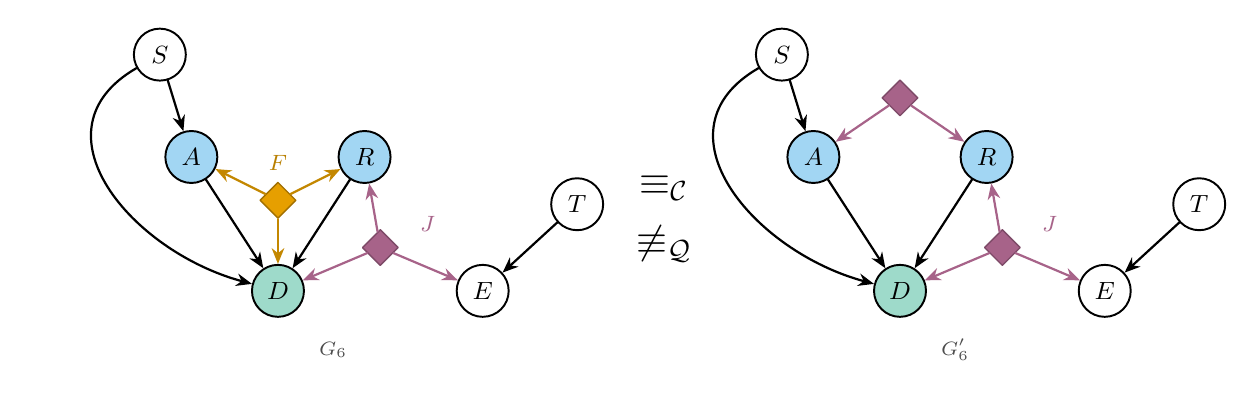
\begin{tikzpicture}[mdag]
  \begin{scope}
    \vn{s}{-0.4,3.0}{$S$} \vn[Cn]{A}{0,1.7}{$A$} \vn[Cn]{R}{2.2,1.7}{$R$} \vn[Dn]{D}{1.1,0}{$D$} \vn{E}{3.7,0}{$E$}
    \vn{t}{4.9,1.1}{$T$}
    \qs[splitsrc]{f}{1.1,1.15} \qs{g}{2.4,0.55}
    \feed[splitedge]{f}{A,R,D} \feed{g}{R,D,E}
    \de{A}{D} \de{R}{D} \de{s}{A} \de{t}{E}
    \draw[edge] (s) to[out=-150,in=165,looseness=1.3] (D);
    \node[lab,text=splitcol!80!black] at (1.1,1.62) {$F$}; \node[lab,text=qcol] at (3.0,0.85) {$J$};
    \node[tag] at (1.8,-0.75) {$\G_6$};
  \end{scope}
  \node[rel] at (6.0,1.3) {$\ceq$};
  \node[rel] at (6.0,0.6) {$\not\qeq$};
  \begin{scope}[shift={(7.9,0)}]
    \vn{s}{-0.4,3.0}{$S$} \vn[Cn]{A}{0,1.7}{$A$} \vn[Cn]{R}{2.2,1.7}{$R$} \vn[Dn]{D}{1.1,0}{$D$} \vn{E}{3.7,0}{$E$}
    \vn{t}{4.9,1.1}{$T$}
    \qs{f}{1.1,2.45} \qs{g}{2.4,0.55}
    \feed{f}{A,R} \feed{g}{R,D,E}
    \de{A}{D} \de{R}{D} \de{s}{A} \de{t}{E}
    \draw[edge] (s) to[out=-150,in=165,looseness=1.3] (D);
    \node[lab,text=qcol] at (3.0,0.85) {$J$};
    \node[tag] at (1.8,-0.75) {$\G_6'$};
  \end{scope}
\end{tikzpicture}
\caption{In both structures the relay belongs to $J$. Splitting $F$ removes Dan from Alice's source, even though Dan still sees Alice, her setting and the relay.}
\label{fig:sixnode}
\end{figure}

Dan ($D$) sees Alice ($A$), the relay ($R$) and Alice's setting $S$. Classically he can sample the latent of $F$ from its posterior
given these data and the latent of $J$ \cite{AWS}. The relay belongs to both sources and can measure its two shares jointly.
In the unsplit structure a relay measurement followed by Alice's measurement can leave Dan entangled with Eve ($E$), outside $F$.

\begin{figure}[H]
\centering
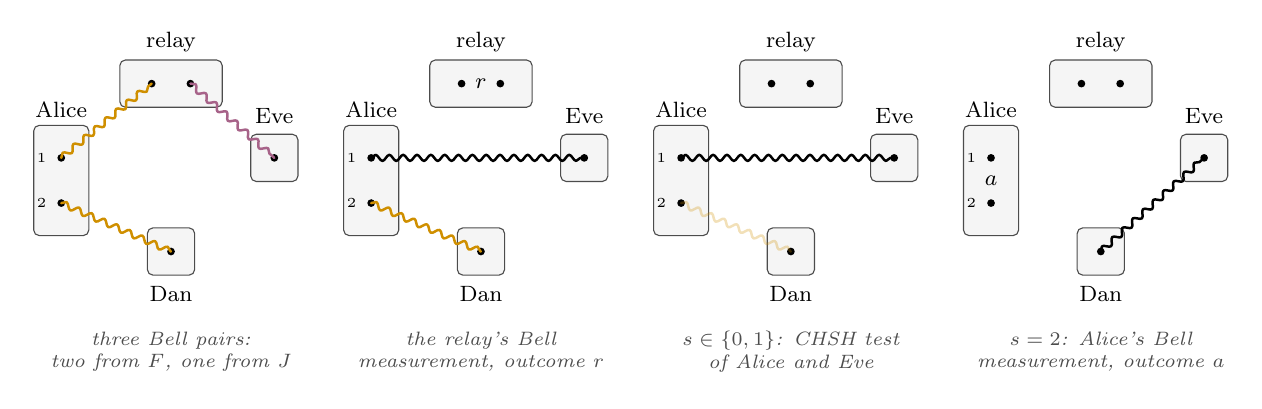
\begin{tikzpicture}[mdag,scale=0.82]
  \tikzset{link/.style={decorate, decoration={snake, amplitude=1.1pt, segment length=5pt}, line width=0.9pt},
           party/.style={draw=black!70, rounded corners=2pt, fill=black!4}}
  \newcommand{\parties}{
    \node[party, minimum width=7mm, minimum height=14mm] at (0,0.8) {}; \node[lab] at (0,1.9) {Alice};
    \coordinate (a1) at (0,1.15); \coordinate (a2) at (0,0.45);
    \node[party, minimum width=13mm, minimum height=6mm] at (1.7,2.3) {}; \node[lab] at (1.7,2.95) {relay};
    \coordinate (r1) at (1.4,2.3); \coordinate (r2) at (2.0,2.3);
    \node[party, minimum width=6mm, minimum height=6mm] at (3.3,1.15) {}; \node[lab] at (3.3,1.8) {Eve};
    \coordinate (e) at (3.3,1.15);
    \node[party, minimum width=6mm, minimum height=6mm] at (1.7,-0.3) {}; \node[lab] at (1.7,-0.95) {Dan};
    \coordinate (d) at (1.7,-0.3);
    \foreach \q in {a1,a2,r1,r2,e,d} { \fill (\q) circle (1.7pt); }
    \node[font=\tiny,anchor=east] at (-0.08,1.15) {1}; \node[font=\tiny,anchor=east] at (-0.08,0.45) {2};}
  \begin{scope}
    \parties
    \draw[link, splitcol!90!black] (a1) -- (r1); \draw[link, splitcol!90!black] (a2) -- (d); \draw[link, qcol] (r2) -- (e);
    \node[tag,align=center] at (1.7,-1.85) {three Bell pairs:\\ two from $F$, one from $J$};
  \end{scope}
  \begin{scope}[shift={(4.8,0)}]
    \parties
    \draw[link] (a1) -- (e); \draw[link, splitcol!90!black] (a2) -- (d);
    \node[lab] at (1.7,2.3) {$r$};
    \node[tag,align=center] at (1.7,-1.85) {the relay's Bell\\ measurement, outcome $r$};
  \end{scope}
  \begin{scope}[shift={(9.6,0)}]
    \parties
    \draw[link] (a1) -- (e); \draw[link, splitcol!90!black, faint] (a2) -- (d);
    \node[tag,align=center] at (1.7,-1.85) {$s\in\{0,1\}$: CHSH test\\ of Alice and Eve};
  \end{scope}
  \begin{scope}[shift={(14.4,0)}]
    \parties
    \draw[link] (d) -- (e);
    \node[lab] at (0,0.8) {$a$};
    \node[tag,align=center] at (1.7,-1.85) {$s=2$: Alice's Bell\\ measurement, outcome $a$};
  \end{scope}
\end{tikzpicture}
\caption{The strategy that produces $P^{*}$ in $\G_6$. Wavy lines are Bell pairs; black dots are qubits. The
relay's measurement links Alice to Eve. Alice then either tests CHSH against Eve, or passes the link on to Dan,
for which she needs the pair that $F$ gave her and Dan.}
\label{fig:strategy}
\end{figure}

\paragraph{A witness with two uses for one Bell pair.}
Take independent uniform inputs $s\in\{0,1,2\}$ and $t\in\{0,1\}$. Source $F$ supplies Alice--relay
and Alice--Dan Bell pairs, and $J$ supplies a relay--Eve pair. The relay's Bell measurement swaps
entanglement to Alice and Eve and announces the Bell label $r$. Eve measures $Z$ or $X$ at $t=0,1$.
At $s=0,1$, Alice measures $(Z+X)/\sqrt2$ or $(Z-X)/\sqrt2$ on her first qubit, recording
$0$ for $+1$ and $1$ for $-1$; Dan outputs $+1$. At $s=2$ Alice Bell-measures her two qubits, swapping
entanglement to Dan and Eve. Knowing $r,a$, Dan corrects the sign of his $Z$ outcome.

\Needspace{10\baselineskip}
The proof uses two observable properties, checked numerically in \cref{app:code}.
\begin{description}[leftmargin=1.2cm,style=nextline,itemsep=1pt]
\item[(P1)] $r$ is uniform, and for each $r$ Alice ($s\in\{0,1\}$) and Eve reach the CHSH value $2\sqrt2$, with a
  different pattern of signs for each $r$. Precisely, give Alice the sign $+1$ when $a=0$ and $-1$ otherwise, and
  let $c_r(s,t)$ be the expectation of the product of her sign and Eve's outcome, given $r$, $s$ and $t$. There are
  signs $\varepsilon(r)\in\{\pm1\}^2$, a different pair for each $r$, with
  \[\varepsilon_0c_r(0,0)+\varepsilon_1c_r(0,1)+\varepsilon_0c_r(1,0)-\varepsilon_1c_r(1,1)=2\sqrt2 .\]
\item[(P2)] at $s=2$, $t=0$: $d=e$ with probability one, and $e$ is uniform given $(r,a)$.
\end{description}

In particular, at $s=2$ Dan predicts a bit that is still uniform to anyone knowing only $(r,a)$.
We use the following exact form of CHSH rigidity \cite{SW}, proved in \cref{app:rigidity}.

\begin{lemma}[CHSH rigidity]\label{lem:rigidity}
Let $A_0,A_1$ be Hermitian operators on $\Hil_A$ and $E_0,E_1$ Hermitian operators on $\Hil_E$, all with square
$\id$, and let $\Hil_{\mathrm{ext}}$ be a further system; all spaces are finite-dimensional. For
$\varepsilon\in\{\pm1\}^2$ put
$W_\varepsilon=A_0\otimes(\varepsilon_0E_0+\varepsilon_1E_1)+A_1\otimes(\varepsilon_0E_0-\varepsilon_1E_1)$, and
suppose that for each $\varepsilon$ there is a state $\omega_\varepsilon$ on
$\Hil_A\otimes\Hil_E\otimes\Hil_{\mathrm{ext}}$ with
$\Tr[W_\varepsilon\,\omega_\varepsilon]=2\sqrt2$. Let $V_A\subseteq\Hil_A$ and $V_E\subseteq\Hil_E$ be the spans of
the supports of the reduced states of the $\omega_\varepsilon$. Then $V_A\cong\mathbb{C}^2\otimes\Hil_{A''}$ and
$V_E\cong\mathbb{C}^2\otimes\Hil_{E''}$ in such a way that on these subspaces
\[
A_0=\tfrac{Z+X}{\sqrt2}\otimes\id,\quad A_1=\tfrac{Z-X}{\sqrt2}\otimes\id,\quad E_0=Z\otimes\id,\quad E_1=X\otimes\id,
\qquad\text{and}\qquad \omega_\varepsilon=\proj{\beta_\varepsilon}\otimes\gamma_\varepsilon ,
\]
where $\beta_\varepsilon$ is the Bell state of two qubits with $Z\otimes Z=\varepsilon_0$ and
$X\otimes X=\varepsilon_1$, and $\gamma_\varepsilon$ is a state on
$\Hil_{A''}\otimes\Hil_{E''}\otimes\Hil_{\mathrm{ext}}$.
\end{lemma}

\begin{proof}[Proof of \cref{thm:sixnode}]
Classical equality follows from the moderate rule, and the witness above belongs to $\Q(\G_6)$.
Suppose a model of $\G_6'$ reproduces it. The independent sources have states $\rho_{AR_1}$ and
$\rho_{R_2DE}$. Alice's first two binary measurements (coarse-graining $a\ne0$) and Eve's two
measurements may be taken projective: use a private pure ancilla for each measurement, including it
in that party's source. This preserves source independence and leaves Alice's $s=2$ measurement available.

\emph{Average over the relay.} Its measurement on $R_1R_2$ leaves a conditional state $\omega_r$ on
$ADE$. Completeness of its POVM and independence of the sources give
$\sum_r p_r\omega_r=\rho_A\otimes\rho_{DE}$. By (P1), $p_r=1/4$ and the four conditioned states
attain the four signed CHSH maxima with the same observables.

\emph{Resolve the four Bell labels.} By \cref{lem:rigidity} the same qubit factors $A',E'$ work for
all $r$ on the supports of the averaged marginals. Eve's observables act as $Z$ and $X$ on $E'$ alone.
The conditional states are $\omega_r=\proj{\beta_r}_{A'E'}\otimes\gamma_r$ on those supports, hence
\[
 \tfrac14\sum_r\proj{\beta_r}_{A'E'}\otimes\gamma_r=\rho_A\otimes\rho_{DE}.
\]
Both Bell marginals are maximally mixed. Taking marginals of this identity gives
$\rho_A=\id_{A'}/2\otimes\alpha_{A''}$ and $\rho_{DE}=\id_{E'}/2\otimes\eta_{E''D}$.
Projecting onto each of the four orthogonal Bell states now gives $\gamma_r=\alpha\otimes\eta$
for every $r$.

\emph{Test Dan's prediction.} At $s=2$ Alice can measure both $A'$ and $A''$. Conditional on $(r,a)$,
this can steer $E'$, but leaves it in product with $\eta_{E''D}$. Eve measures $Z$ on $E'$ at $t=0$,
so her outcome is independent of Dan's given $(r,a)$. By (P2) that outcome is uniform, making their
agreement probability $1/2$ instead of one. This excludes the witness from $\Q(\G_6')$.
\end{proof}

The four-valued relay matters here. It identifies each Bell state uniquely, which is why the projection
fixes every $\gamma_r$. With sixteen outcomes the relay could swap two pairs and report two results.
Several labels would then give the same CHSH signs, and the projection would fix only their sum.

\paragraph{Four-node splits.}\label{sec:open-four}
On four nodes there are five groups for which the classical strong rule licenses a split and the
quantum rules give no such equivalence. The six-node witness uses an independent setting on each side and four different relay outcomes.
The four-node groups leave no room for the extra setting nodes. In the last two groups every node of
$C$ also belongs to a remaining source. Whether any of these splits preserves $\Q$ is open.

\begin{figure}[!htb]
\centering
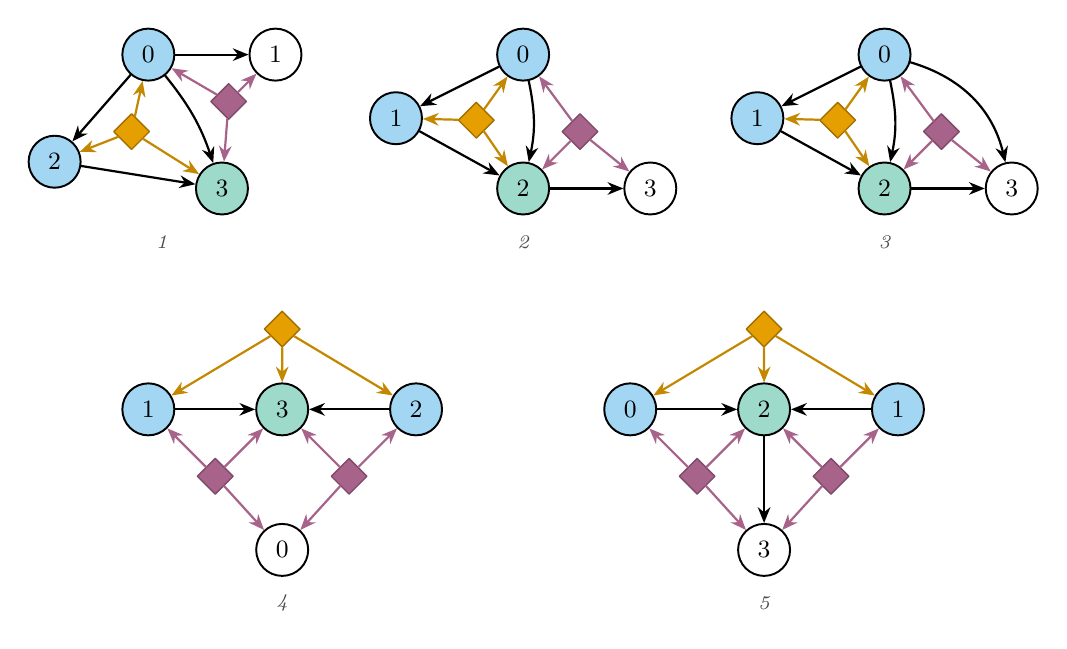
\begin{tikzpicture}[mdag,scale=0.85]
  % group 1
  \begin{scope}
    \vn[Cn]{n0}{1.2,1.9}{$0$} \vn{n1}{3.1,1.9}{$1$} \vn[Cn]{n2}{-0.2,0.3}{$2$} \vn[Dn]{n3}{2.3,-0.1}{$3$}
    \qs[splitsrc]{f}{0.95,0.75} \qs{g}{2.4,1.2}
    \feed[splitedge]{f}{n0,n2,n3} \feed{g}{n0,n1,n3}
    \de{n0}{n1} \de{n0}{n2} \de{n2}{n3} \draw[edge] (n0) to[bend left=10] (n3);
    \node[tag] at (1.4,-0.9) {1};
  \end{scope}
  % groups 2 and 3
  \foreach \shift/\name in {5.6/2, 11.0/3} {
  \begin{scope}[shift={(\shift,0)}]
    \vn[Cn]{n0}{1.2,1.9}{$0$} \vn[Cn]{n1}{-0.7,0.95}{$1$} \vn[Dn]{n2}{1.2,-0.1}{$2$} \vn{n3}{3.1,-0.1}{$3$}
    \qs[splitsrc]{f}{0.5,0.92} \qs{g}{2.05,0.75}
    \feed[splitedge]{f}{n0,n1,n2} \feed{g}{n0,n2,n3}
    \de{n0}{n1} \de{n1}{n2} \de{n2}{n3} \draw[edge] (n0) to[bend left=12] (n2);
    \node[tag] at (1.2,-0.9) {\name};
  \end{scope}}
  \draw[edge] (n0) to[bend left=30] (n3);   % group 3 only: the nodes of the last panel drawn
  % groups 4 and 5: the green node is a member of all three sources
  \begin{scope}[shift={(1.2,-4.6)}]
    \vn[Cn]{n1}{0,1.2}{$1$} \vn[Cn]{n2}{4,1.2}{$2$} \vn[Dn]{n3}{2,1.2}{$3$} \vn{n0}{2,-0.9}{$0$}
    \qs[splitsrc]{f}{2,2.4} \qs{g1}{1.0,0.2} \qs{g2}{3.0,0.2}
    \feed[splitedge]{f}{n1,n2,n3} \feed{g1}{n0,n1,n3} \feed{g2}{n0,n2,n3}
    \de{n1}{n3} \de{n2}{n3}
    \node[tag] at (2,-1.7) {4};
  \end{scope}
  \begin{scope}[shift={(8.4,-4.6)}]
    \vn[Cn]{n0}{0,1.2}{$0$} \vn[Cn]{n1}{4,1.2}{$1$} \vn[Dn]{n2}{2,1.2}{$2$} \vn{n3}{2,-0.9}{$3$}
    \qs[splitsrc]{f}{2,2.4} \qs{g1}{1.0,0.2} \qs{g2}{3.0,0.2}
    \feed[splitedge]{f}{n0,n1,n2} \feed{g1}{n0,n2,n3} \feed{g2}{n1,n2,n3}
    \de{n0}{n2} \de{n1}{n2} \de{n2}{n3}
    \node[tag] at (2,-1.7) {5};
  \end{scope}
\end{tikzpicture}
\caption{The largest structure of each open group. The strong rule splits the orange source into the blue and green parts. In each graph a blue node also belongs to a remaining source.}
\label{fig:open-four}
\end{figure}


\clearpage
\section{Gaps, classes and the census}\label{sec:buys}

\subsection{A gap is a property of the class}

\begin{proposition}\label{prop:class}
Each rule of Part~I (\cref{lem:monotone} used in both directions, \cref{thm:split,thm:ruleA,thm:ruleB}) preserves
the quantum model set \emph{and} the classical model set. Hence, if $\G$ and $\G'$ are connected by these rules,
then $\G$ has a QC gap if and only if $\G'$ has one.
\end{proposition}
\begin{proof}
$\Q(\G)=\Q(\G')$ and $\C(\G)=\C(\G')$, so $\Q(\G)\not\subseteq\C(\G)$ is the same statement for both.
\end{proof}

This is the whole reason for classifying. It should be compared with what a \emph{classical} equivalence gives,
which is less.

\begin{lemma}[The upward rule]\label{lem:upward}
Let $\C(\G')=\C(\G)$ and let $\G'$ be structurally above $\G$ (more edges, larger sources). If $\G$ has a QC gap,
so has $\G'$.
\end{lemma}
\begin{proof}
$\Q(\G')\supseteq\Q(\G)\not\subseteq\C(\G)=\C(\G')$, the first step by \cref{lem:monotone}.
\end{proof}

Whether a gap also passes \emph{downward} inside a classical class is not known, and
\cref{thm:hlp-four,thm:sixnode} show why it is not automatic: within one classical class the quantum model set can
shrink strictly.

\subsection{The four-node census in numbers}

The repository enumerates all structures on three and on four visible nodes up to relabelling, with every source
quantum, and builds two graphs on them (\code{metagraph\_advanced.py}). In the \emph{quantum metagraph} the edges
are structural dominance and the rules of Part~I; in the \emph{classical metagraph} they are structural dominance,
the classical edge rule and strong face splitting. The strongly connected components are proven equivalence
classes, quantum and classical respectively. ``Proven'' is meant literally: two different classes may still be
equivalent by an argument that no rule captures.

\begin{center}
\small
\renewcommand{\arraystretch}{1.2}
\begin{tabular}{@{}lrr@{}}
\toprule
 & three nodes & four nodes\\
\midrule
structures up to relabelling & 46 & 2809\\
classical classes & 8 & 396\\
\quad of which contain a structure without sources & 5 & 20\\
quantum classes with the rules of Part~I & 8 & \textbf{446}\\
\quad for comparison, with strong face splitting (unsound) & 8 & 438\\
\quad for comparison, with weak face splitting only & 8 & 461\\
input classes of the census, and the structures in them & 3,\ 5 & 426,\ 996\\
\quad with a proven QC gap & 3,\ 5 & 380,\ 935\\
\quad open & 0 & 46,\ 61\\
\bottomrule
\end{tabular}
\end{center}

\emph{Inputs.} A class that contains a structure classically equivalent to one without sources cannot have a gap:
its classical model set is everything that satisfies the conditional independences read off the graph, and
quantum models satisfy those as well \cite{HLP}. The other $426$ quantum classes are the inputs of the census.

\emph{How a gap is proved.} A few structures have a gap by a direct argument; they are the \emph{seeds}: the
instrumental scenario, the Evans scenario, the triangle, and the Bell scenario with independent or with linked
settings (\code{known\_QC\_gaps.py}). Every other proof is a chain of \emph{reductions} that ends at a seed. A
reduction is a map from a structure $\G$ to a smaller or simpler structure $\G_0$ together with a proof that a gap
of $\G_0$ implies a gap of $\G$. Such a proof always has two halves, and the repository names them:
\begin{itemize}
\item \emph{the quantum direction}: a quantum model of $\G$ can produce every quantum distribution of $\G_0$, in a
  form that has the extra observable properties the step relies on (for instance, one node perfectly predicts
  another);
\item \emph{the classical direction}: if a distribution with those properties were classical in $\G$, the
  corresponding distribution would be classical in $\G_0$.
\end{itemize}
The reductions used are: fixing a node to a constant, marginalising a node, postselecting on a node, stitching two
nodes into one, making a quantum source classical (\emph{degradation}), and a family of steps due to Fritz in
which a node whose outcome another node predicts loses the parents that the predictor does not see. They are
described in \code{manuscript/piggybacks.md}. An equivalence is the degenerate reduction in which both directions
are identities.

\emph{What changed with the sound rule.} Restricting face splitting to \cref{thm:split} separates five classes
into $13$ (\cref{sec:open-four}). All $13$ have a gap, by fixing a node to a constant or by the upward rule, so the
proven classes go from $372$ to $380$ and the open classes are the same $46$ as before, with the same $61$
structures.

\subsection{Gaps that are reached only through equivalence}\label{sec:only-via}

How much of the census actually rests on \cref{prop:class}? To find out, the search was run on each of the $996$
structures of the input classes separately, so that no step may replace a structure by an equivalent one
(\code{scripts/only\_via\_equivalence.py}).

\begin{center}
\small
\renewcommand{\arraystretch}{1.2}
\begin{tabular}{@{}p{8.2cm}rr@{}}
\toprule
what the search may use, besides the reductions & structures reached & not reached\\
\midrule
all seeds, classes as in the census & 935 & \\
all seeds, no equivalence of any kind & 933 & \textbf{2}\\
all seeds, classical equivalence in the upward rule only & 934 & \textbf{1}\\
\bottomrule
\end{tabular}
\end{center}

The numbers are the same for the ten-stage search and for the deeper search that is now the default of the
repository (one Fritz step that may grow the structure up to six nodes). The two structures that no reduction
reaches lie in one class, the Bell scenario with linked settings, shown in \cref{fig:bell-class}.

\begin{figure}[H]
\centering
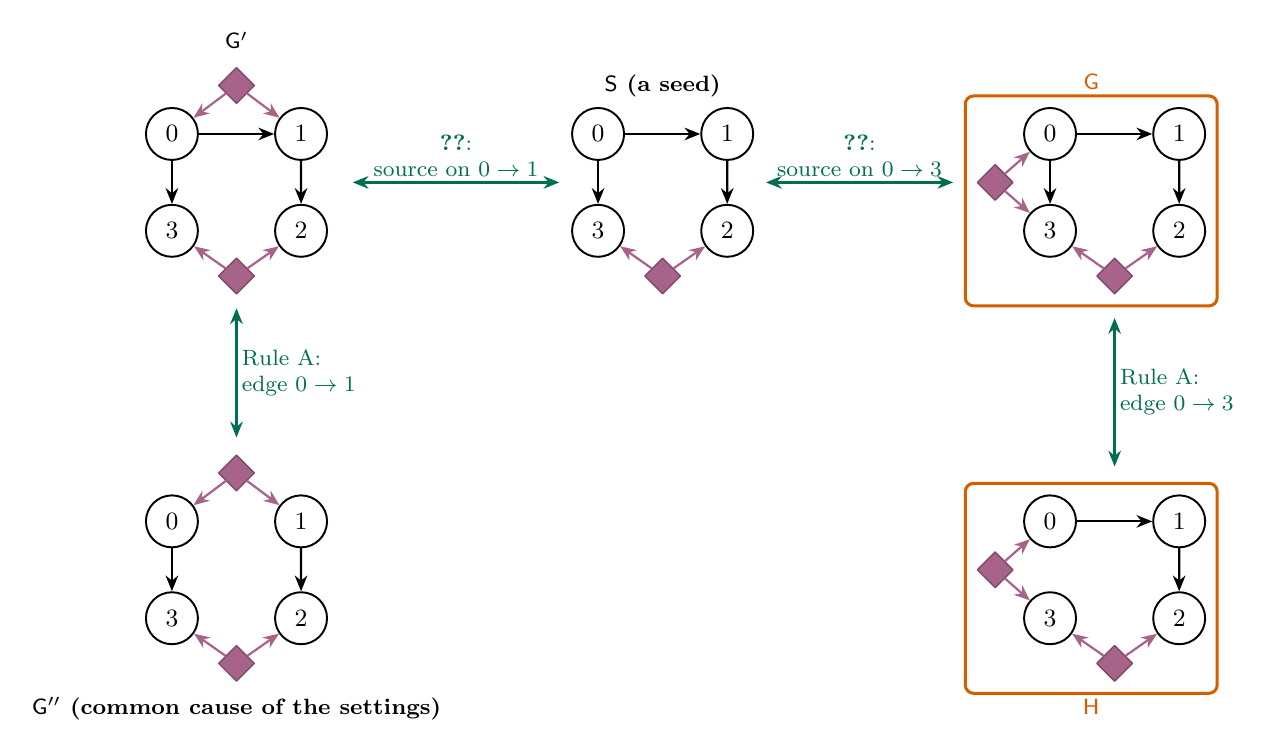
\begin{tikzpicture}[mdag,scale=0.82]
  % in every picture: settings 0 (top left) and 1 (top right), outcomes 3 (bottom left) and 2 (bottom right)
  \newcommand{\bellnodes}{\vn{x}{0,1.5}{$0$} \vn{y}{2,1.5}{$1$} \vn{a}{0,0}{$3$} \vn{b}{2,0}{$2$} \qs{q}{1,-0.7} \feed{q}{a,b}}
  % --- G' (top left)
  \begin{scope}[shift={(0,4.4)}]
    \bellnodes \qs{l}{1,2.25} \feed{l}{x,y} \de{x}{y} \de{x}{a} \de{y}{b}
    \node[lab,font=\footnotesize\bfseries] at (1,2.95) {$\mathsf{G}'$};
  \end{scope}
  % --- S (top centre)
  \begin{scope}[shift={(6.6,4.4)}]
    \bellnodes \de{x}{y} \de{x}{a} \de{y}{b}
    \node[lab,font=\footnotesize\bfseries] at (1,2.25) {$\mathsf{S}$ (a seed)};
  \end{scope}
  % --- G (top right)
  \begin{scope}[shift={(13.6,4.4)}]
    \bellnodes \qs{l}{-0.85,0.75} \feed{l}{x,a} \de{x}{y} \de{x}{a} \de{y}{b}
    \begin{scope}[on background layer]
      \node[draw=oired, line width=1.1pt, rounded corners=3pt, fit=(x)(y)(a)(b)(q)(l), inner sep=4pt] (frameG) {};
    \end{scope}
    \node[lab,font=\footnotesize\bfseries,text=oired,anchor=south] at (frameG.north) {$\mathsf{G}$};
  \end{scope}
  % --- G'' (bottom left)
  \begin{scope}[shift={(0,-1.6)}]
    \bellnodes \qs{l}{1,2.25} \feed{l}{x,y} \de{x}{a} \de{y}{b}
    \node[lab,font=\footnotesize\bfseries] at (1,-1.4) {$\mathsf{G}''$ (common cause of the settings)};
  \end{scope}
  % --- H (bottom right)
  \begin{scope}[shift={(13.6,-1.6)}]
    \bellnodes \qs{l}{-0.85,0.75} \feed{l}{x,a} \de{x}{y} \de{y}{b}
    \begin{scope}[on background layer]
      \node[draw=oired, line width=1.1pt, rounded corners=3pt, fit=(x)(y)(a)(b)(q)(l), inner sep=4pt] (frameH) {};
    \end{scope}
    \node[lab,font=\footnotesize\bfseries,text=oired,anchor=north] at (frameH.south) {$\mathsf{H}$};
  \end{scope}
  % --- equivalences, labelled by the rule that proves them
  \draw[<->, line width=0.9pt, oigreen!70!black] (2.8,5.15) -- node[lab,above,align=center] {\cref{thm:split}:\\ source on $0\to1$} (6.0,5.15);
  \draw[<->, line width=0.9pt, oigreen!70!black] (9.2,5.15) -- node[lab,above,align=center] {\cref{thm:split}:\\ source on $0\to3$} (12.1,5.15);
  \draw[<->, line width=0.9pt, oigreen!70!black] (1.0,3.2) -- node[lab,right,align=left] {Rule A:\\ edge $0\to1$} (1.0,1.2);
  \draw[<->, line width=0.9pt, oigreen!70!black] (14.6,3.05) -- node[lab,right,align=left] {Rule A:\\ edge $0\to3$} (14.6,0.75);
\end{tikzpicture}
\caption{The class of the Bell scenario with linked settings: settings $0$ and $1$, outcomes $3$ and $2$. Green
arrows are equivalences, labelled by the rule that proves them. In the repository's notation:
$\mathsf{S}=$ \str{0→1, 0→3, 1→2; Q\{2,3\}}; $\mathsf{G}'=\mathsf S$ with \str{Q\{0,1\}};
$\mathsf{G}''=$ \str{0→3, 1→2; Q\{0,1\}, Q\{2,3\}}; $\mathsf{G}=\mathsf S$ with \str{Q\{0,3\}};
$\mathsf{H}=$ \str{0→1, 1→2; Q\{0,3\}, Q\{2,3\}}. The two framed structures are reached by no reduction.}
\label{fig:bell-class}
\end{figure}

How each member gets its gap:
\begin{itemize}
\item $\mathsf S$ is a seed. Its gap is Bell's theorem with correlated settings: the source of the outcomes is
  independent of both settings, so any classical model is local for $P(x_3,x_2\mid x_0,x_1)$.
\item $\mathsf{G}'$ and $\mathsf{G}''$, in which the settings share a quantum common cause, follow from seeds by
  degradation: making that common cause classical gives the Bell scenario with a classical link between the
  settings, which is a seed by the same direct argument.
\item $\mathsf G$ follows from $\mathsf S$ by the upward rule (\cref{lem:upward}), which uses the \emph{classical}
  equivalence of the two; with no equivalence at all it is not reached.
\item $\mathsf H$ is reached in no other way than through its quantum equivalence with $\mathsf G$ (Rule A), and
  from there with $\mathsf S$ (\cref{thm:split}).
\end{itemize}

In $\mathsf H$ the outcome $3$ learns its setting $0$ only through a quantum source. No reduction turns a source
into an edge: reductions remove nodes, remove parents or make sources classical. Turning that source into an edge
is exactly what Rule A does, because the setting is premeasurable.

Two further facts put this class in perspective (same script).
\begin{itemize}
\item \emph{The class is not reachable from the other seeds at all.} If the three seeds with linked settings are
  left out, no member of the class is proven, with or without equivalence ($379$ classes and $930$ structures
  remain proven). No reduction leads from a Bell scenario with linked settings to one with independent settings,
  since removing the link is not a reduction. The class needs its own direct argument; equivalence then spreads
  it to all five members.
\item \emph{Elsewhere equivalence is a convenience.} In every other proven class, each member is reached by
  reductions on its own. What the classes buy there is economy and certainty: $426$ problems instead of $996$, one
  certificate per class, and the assurance that counting classes does not count the same problem twice.
\end{itemize}

\subsection{A classical source that is as good as a quantum one}

The seeds are often stated with some sources classical, for instance the Bell scenario in which each party
receives its setting through a classical common cause. Structures with some sources declared classical are called
\emph{hybrids}; in a model of a hybrid the states of the classical sources are diagonal. Pre-measurement tells when
the declaration makes no difference.

\begin{proposition}[\code{QmDAG.lift}]\label{prop:lift}
Let $F$ be a source of a hybrid all of whose members, except at most one, are premeasurable. Then declaring $F$
classical or quantum gives the same quantum model set.
\end{proposition}
\begin{proof}
Let $F$ be quantum and apply \cref{lem:premeasure} to each premeasurable member. Every member then holds the
outcomes $\ell$ of all of them, and what is left of the state is a state $\rho_m(\ell)$ of the one remaining member
$m$, labelled by $\ell$. That member can prepare $\rho_m(\ell)$ itself once it knows $\ell$. So $F$ only needs to
distribute $\ell$, which is classical.
\end{proof}

With this, the nine Bell seeds of the repository are two classes (independent settings, linked settings) and the
three instrumental seeds are one.

\subsection{What a new quantum-valid rule would buy}

Three statements are left open by this note.
\begin{enumerate}[leftmargin=*]
\item The edge rule when an other member of the origin's source has two sources and no visible parent (the open
  box at the end of \cref{sec:edge}).
\item The five four-node splits of \cref{sec:open-four}.
\item Whether a gap passes downward inside a classical class.
\end{enumerate}
None of them can help the $46$ open classes, and this can be read off the classification. Of the $396$ classical
classes on four nodes, $374$ contain a single quantum class and $22$ contain several ($2$ to $9$); all $22$ are
entirely proven. Every open class is the only quantum class of its classical class. So even the full classical
rules, were they valid, would not connect an open class to a proven one. A rule that helps must be new classically
as well.

What equivalence already does for the open classes is to shrink them: the $46$ classes hold $61$ structures, and
the largest holds $12$. A gap for one member is a gap for all.


\appendix
\section{Reproducing the figures and counts}\label{app:code}
Run the scripts below from the note's directory. Each writes its results to \code{scripts/output/}.
The rule checks call the same edge-dropping and closed-family splitting methods as the census.
\begin{center}
\small
\begin{tabular}{@{}ll@{}}
\toprule
Result & Script in \code{scripts/}\\
\midrule
Rule hypotheses and examples & \code{check\_examples.py}\\
Equivalence class counts & \code{class\_counts.py} (\code{--five} adds five nodes)\\
Census totals and open classes & \code{census\_facts.py}\\
Six-node Bell strategy, (P1) and (P2) & \code{six\_node\_strategy.py}\\
Four-node search with equivalence switched off & \code{only\_via\_equivalence.py}\\
Five-node piggyback certificate and four moves & \code{bell\_piggyback.py}\\
\bottomrule
\end{tabular}
\end{center}
The named seeds are in \code{known\_QC\_gaps.py}. To rebuild the PDF, run \code{./build.sh}.

\section{Proof of the rigidity lemma}\label{app:rigidity}

This appendix proves \cref{lem:rigidity}. The notation is that of the lemma: $A_0,A_1$ on $\Hil_A$ and $E_0,E_1$
on $\Hil_E$ are Hermitian with square $\id$, and
$W_\varepsilon=A_0\otimes(\varepsilon_0E_0+\varepsilon_1E_1)+A_1\otimes(\varepsilon_0E_0-\varepsilon_1E_1)$.

\begin{proof}[Proof of \cref{lem:rigidity}]
Fix $\varepsilon$, write $\omega=\omega_\varepsilon$, and put
$\tilde E_0=(\varepsilon_0E_0+\varepsilon_1E_1)/\sqrt2$, $\tilde E_1=(\varepsilon_0E_0-\varepsilon_1E_1)/\sqrt2$.
Using $A_s^2=E_t^2=\id$ and that the $A$'s commute with the $E$'s,
\[
2\sqrt2\,\id-W_\varepsilon=\tfrac{1}{\sqrt2}\bigl[(A_0-\tilde E_0)^2+(A_1-\tilde E_1)^2\bigr].
\]
Both squares are positive, so $\Tr[W_\varepsilon\omega]=2\sqrt2$ forces $\Tr[(A_s-\tilde E_s)^2\omega]=0$, hence
\begin{equation}\label{eq:rig}
A_s\,\omega=\tilde E_s\,\omega\qquad(s=0,1).
\end{equation}
\emph{Anticommutation.} From \eqref{eq:rig},
$\omega=A_0^2\omega=A_0\tilde E_0\omega=\tilde E_0A_0\omega=\tilde E_0^2\omega$, and
$\tilde E_0^2=\id+\tfrac12\varepsilon_0\varepsilon_1\{E_0,E_1\}$, so $\{E_0,E_1\}\,\omega=0$. Likewise
$\{A_0,A_1\}\omega=(\tilde E_1A_0+\tilde E_0A_1)\omega=\{\tilde E_0,\tilde E_1\}\omega=(E_0^2-E_1^2)\omega=0$.

\emph{Invariant supports.} Adding the two equations \eqref{eq:rig} gives $E_0\,\omega=\varepsilon_0\,L\omega$ with
$L=(A_0+A_1)/\sqrt2$ acting on $\Hil_A$, and, taking adjoints, $\omega E_0=\varepsilon_0\,\omega L$. Let $\omega_E$
be the reduced state on $\Hil_E$. Then
\[
E_0\,\omega_E\,E_0=\Tr_{A,\mathrm{ext}}[E_0\,\omega\,E_0]=\Tr_{A,\mathrm{ext}}[L\omega L]=\Tr_{A,\mathrm{ext}}[L^2\omega]
\le\lVert L\rVert^2\,\omega_E ,
\]
where the third equality holds because $L$ acts on a system that is traced out, and the inequality because
$\Tr_{A,\mathrm{ext}}[(\lVert L\rVert^2\id-L^2)\,\omega]=\Tr_{A,\mathrm{ext}}[N\omega N]\ge0$ for the positive
square root $N$ of $\lVert L\rVert^2\id-L^2$. So $E_0$ maps the support of $\omega_E$ into itself, and so does
$E_1$; symmetrically $A_0,A_1$ preserve the support of $\omega_A$. Taking the partial trace of
$\{E_0,E_1\}\omega=0$ gives $\{E_0,E_1\}\omega_E=0$, so $E_0$ and $E_1$ anticommute on the support of $\omega_E$,
and likewise $A_0,A_1$ on the support of $\omega_A$. All of this holds for every $\varepsilon$, hence on the spans
$V_E$ and $V_A$.

\emph{Qubits.} Two anticommuting Hermitian operators with square $\id$ on a finite-dimensional space $V$ are
$Z\otimes\id$ and $X\otimes\id$ for a suitable identification $V\cong\mathbb{C}^2\otimes V''$: the second maps the
$+1$ eigenspace of the first isometrically onto its $-1$ eigenspace. Apply this to $E_0,E_1$ on $V_E$ and to
$(A_0+A_1)/\sqrt2,\ (A_0-A_1)/\sqrt2$ on $V_A$, which also anticommute and square to $\id$ there.

\emph{The state.} In these coordinates $W_\varepsilon=\sqrt2\,(\varepsilon_0\,Z\otimes Z+\varepsilon_1\,X\otimes X)\otimes\id$
on $V_A\otimes V_E\otimes\Hil_{\mathrm{ext}}$. The operators $Z\otimes Z$ and $X\otimes X$ commute and are jointly
diagonal in the Bell basis, so the largest eigenvalue $2\sqrt2$ of $\sqrt2(\varepsilon_0ZZ+\varepsilon_1XX)$ is
attained on $\beta_\varepsilon$ only. As $\omega$ is supported on $V_A\otimes V_E\otimes\Hil_{\mathrm{ext}}$ and
attains this eigenvalue in expectation, $\omega=\proj{\beta_\varepsilon}\otimes\gamma_\varepsilon$.
\end{proof}


\begin{thebibliography}{99}

\bibitem{AWS} M.~M.~Ansanelli, E.~Wolfe and R.~W.~Spekkens, \emph{The observational partial order of causal
structures with latent variables}, arXiv:2502.07891. The classical facet-adding rules (Propositions 5, 7 and 8; the
proof of the strong rule is in Appendix A) and the edge rule in the form used here (Proposition 4).

\bibitem{Evans} R.~J.~Evans, \emph{Graphs for margins of Bayesian networks}, Scand.\ J.\ Stat.\ \textbf{43}, 625
(2016). mDAGs; the original face-splitting rule (Proposition 6.1 of the arXiv version).

\bibitem{HLP} J.~Henson, R.~Lal and M.~F.~Pusey, \emph{Theory-independent limits on correlations from generalized
Bayesian networks}, New J.\ Phys.\ \textbf{16}, 113043 (2014). The edge rule; observable d-separation holds in
quantum theory.

\bibitem{Fritz} T.~Fritz, \emph{Beyond Bell's theorem: correlation scenarios}, New J.\ Phys.\ \textbf{14}, 103001
(2012). The triangle distribution used in \cref{thm:hlp-four}.

\bibitem{MAG} Ll.~Masanes, A.~Ac\'{\i}n and N.~Gisin, \emph{General properties of nonsignaling theories},
Phys.\ Rev.\ A \textbf{73}, 012112 (2006). Correlations that can be shared with a second copy of one party are
local; \cref{lem:predict} is the case used here.

\bibitem{Inflation} E.~Wolfe, A.~Pozas-Kerstjens, M.~Grinberg, D.~Rosset, A.~Ac\'{\i}n and M.~Navascu\'es,
\emph{Quantum inflation: a general approach to quantum causal compatibility}, Phys.\ Rev.\ X \textbf{11}, 021043
(2021). Experiments built from independent copies of the sources without cloning, as in the proof of
\cref{thm:hlp-four}.

\bibitem{SW} S.~J.~Summers and R.~Werner, \emph{Maximal violation of Bell's inequalities is generic in quantum
field theory}, Commun.\ Math.\ Phys.\ \textbf{110}, 247 (1987); S.~Popescu and D.~Rohrlich, \emph{Which states
violate Bell's inequality maximally?}, Phys.\ Lett.\ A \textbf{169}, 411 (1992); M.~McKague, T.~H.~Yang and
V.~Scarani, \emph{Robust self-testing of the singlet}, J.\ Phys.\ A \textbf{45}, 455304 (2012). Rigidity of the
maximal CHSH violation; \cref{lem:rigidity} is the exact version, proved in full above.

\bibitem{Repo} \code{manuscript/piggybacks.md} in the \code{mDAG-analysis} repository. The reductions, the seeds
and the four-node census.

\end{thebibliography}


\end{document}
